% Options for packages loaded elsewhere
\PassOptionsToPackage{unicode}{hyperref}
\PassOptionsToPackage{hyphens}{url}
\PassOptionsToPackage{dvipsnames,svgnames*,x11names*}{xcolor}
%
\documentclass[
  10pt,
  dvipsnames,enabledeprecatedfontcommands]{scrartcl}
\usepackage{amsmath,amssymb}
\usepackage{lmodern}
\usepackage{ifxetex,ifluatex}
\ifnum 0\ifxetex 1\fi\ifluatex 1\fi=0 % if pdftex
  \usepackage[T1]{fontenc}
  \usepackage[utf8]{inputenc}
  \usepackage{textcomp} % provide euro and other symbols
\else % if luatex or xetex
  \usepackage{unicode-math}
  \defaultfontfeatures{Scale=MatchLowercase}
  \defaultfontfeatures[\rmfamily]{Ligatures=TeX,Scale=1}
\fi
% Use upquote if available, for straight quotes in verbatim environments
\IfFileExists{upquote.sty}{\usepackage{upquote}}{}
\IfFileExists{microtype.sty}{% use microtype if available
  \usepackage[]{microtype}
  \UseMicrotypeSet[protrusion]{basicmath} % disable protrusion for tt fonts
}{}
\makeatletter
\@ifundefined{KOMAClassName}{% if non-KOMA class
  \IfFileExists{parskip.sty}{%
    \usepackage{parskip}
  }{% else
    \setlength{\parindent}{0pt}
    \setlength{\parskip}{6pt plus 2pt minus 1pt}}
}{% if KOMA class
  \KOMAoptions{parskip=half}}
\makeatother
\usepackage{xcolor}
\IfFileExists{xurl.sty}{\usepackage{xurl}}{} % add URL line breaks if available
\IfFileExists{bookmark.sty}{\usepackage{bookmark}}{\usepackage{hyperref}}
\hypersetup{
  pdftitle={Probability Thresholds},
  pdfauthor={Marcello Di Bello and Rafal Urbaniak},
  colorlinks=true,
  linkcolor=Maroon,
  filecolor=Maroon,
  citecolor=Blue,
  urlcolor=blue,
  pdfcreator={LaTeX via pandoc}}
\urlstyle{same} % disable monospaced font for URLs
\usepackage{graphicx}
\makeatletter
\def\maxwidth{\ifdim\Gin@nat@width>\linewidth\linewidth\else\Gin@nat@width\fi}
\def\maxheight{\ifdim\Gin@nat@height>\textheight\textheight\else\Gin@nat@height\fi}
\makeatother
% Scale images if necessary, so that they will not overflow the page
% margins by default, and it is still possible to overwrite the defaults
% using explicit options in \includegraphics[width, height, ...]{}
\setkeys{Gin}{width=\maxwidth,height=\maxheight,keepaspectratio}
% Set default figure placement to htbp
\makeatletter
\def\fps@figure{htbp}
\makeatother
\setlength{\emergencystretch}{3em} % prevent overfull lines
\providecommand{\tightlist}{%
  \setlength{\itemsep}{0pt}\setlength{\parskip}{0pt}}
\setcounter{secnumdepth}{5}
%\documentclass{article}

% %packages
 \usepackage{booktabs}

\usepackage{multirow}

\usepackage{graphicx}
\usepackage{longtable}
\usepackage{ragged2e}
\usepackage{etex}
%\usepackage{yfonts}
\usepackage{marvosym}
\usepackage[notextcomp]{kpfonts}
\usepackage{nicefrac}
\newcommand*{\QED}{\hfill \footnotesize {\sc Q.e.d.}}
\usepackage{floatrow}

\usepackage[textsize=footnotesize]{todonotes}
%\linespread{1.5}
\newcommand{\indep}{\!\perp \!\!\! \perp\!}


\setlength{\parindent}{10pt}
\setlength{\parskip}{1pt}


%language
\usepackage{times}
\usepackage{t1enc}
%\usepackage[utf8x]{inputenc}
%\usepackage[polish]{babel}
%\usepackage{polski}




%AMS
\usepackage{amsfonts}
\usepackage{amssymb}
\usepackage{amsthm}
\usepackage{amsmath}
\usepackage{mathtools}

\usepackage{geometry}
 \geometry{a4paper,left=35mm,top=20mm,}


%environments
\newtheorem{fact}{Fact}



%abbreviations
\newcommand{\ra}{\rangle}
\newcommand{\la}{\langle}
\newcommand{\n}{\neg}
\newcommand{\et}{\wedge}
\newcommand{\jt}{\rightarrow}
\newcommand{\ko}[1]{\forall  #1\,}
\newcommand{\ro}{\leftrightarrow}
\newcommand{\exi}[1]{\exists\, {_{#1}}}
\newcommand{\pr}[1]{\mathsf{P}(#1)}
\newcommand{\cost}{\mathsf{cost}}
\newcommand{\benefit}{\mathsf{benefit}}
\newcommand{\ut}{\mathsf{ut}}

\newcommand{\odds}{\mathsf{Odds}}
\newcommand{\ind}{\mathsf{Ind}}
\newcommand{\nf}[2]{\nicefrac{#1\,}{#2}}
\newcommand{\R}[1]{\texttt{#1}}
\newcommand{\prr}[1]{\mbox{$\mathtt{P}_{prior}(#1)$}}
\newcommand{\prp}[1]{\mbox{$\mathtt{P}_{posterior}(#1)$}}



\newtheorem{q}{\color{blue}Question}
\newtheorem{lemma}{Lemma}
\newtheorem{theorem}{Theorem}



%technical intermezzo
%---------------------

\newcommand{\intermezzoa}{
	\begin{minipage}[c]{13cm}
	\begin{center}\rule{10cm}{0.4pt}



	\tiny{\sc Optional Content Starts}
	
	\vspace{-1mm}
	
	\rule{10cm}{0.4pt}\end{center}
	\end{minipage}\nopagebreak 
	}


\newcommand{\intermezzob}{\nopagebreak 
	\begin{minipage}[c]{13cm}
	\begin{center}\rule{10cm}{0.4pt}

	\tiny{\sc Optional Content Ends}
	
	\vspace{-1mm}
	
	\rule{10cm}{0.4pt}\end{center}
	\end{minipage}
	}
%--------------------






















\newtheorem*{reply*}{Reply}
\usepackage{enumitem}
\newcommand{\question}[1]{\begin{enumerate}[resume,leftmargin=0cm,labelsep=0cm,align=left]
\item #1
\end{enumerate}}

\usepackage{float}

% \setbeamertemplate{blocks}[rounded][shadow=true]
% \setbeamertemplate{itemize items}[ball]
% \AtBeginPart{}
% \AtBeginSection{}
% \AtBeginSubsection{}
% \AtBeginSubsubsection{}
% \setlength{\emergencystretch}{0em}
% \setlength{\parskip}{0pt}






\usepackage[authoryear]{natbib}

%\bibliographystyle{apalike}



\usepackage{tikz}
\usetikzlibrary{positioning,shapes,arrows}

\ifluatex
  \usepackage{selnolig}  % disable illegal ligatures
\fi
\newlength{\cslhangindent}
\setlength{\cslhangindent}{1.5em}
\newlength{\csllabelwidth}
\setlength{\csllabelwidth}{3em}
\newenvironment{CSLReferences}[2] % #1 hanging-ident, #2 entry spacing
 {% don't indent paragraphs
  \setlength{\parindent}{0pt}
  % turn on hanging indent if param 1 is 1
  \ifodd #1 \everypar{\setlength{\hangindent}{\cslhangindent}}\ignorespaces\fi
  % set entry spacing
  \ifnum #2 > 0
  \setlength{\parskip}{#2\baselineskip}
  \fi
 }%
 {}
\usepackage{calc}
\newcommand{\CSLBlock}[1]{#1\hfill\break}
\newcommand{\CSLLeftMargin}[1]{\parbox[t]{\csllabelwidth}{#1}}
\newcommand{\CSLRightInline}[1]{\parbox[t]{\linewidth - \csllabelwidth}{#1}\break}
\newcommand{\CSLIndent}[1]{\hspace{\cslhangindent}#1}

\title{Probability Thresholds}
\author{Marcello Di Bello and Rafal Urbaniak}
\date{}

\begin{document}
\maketitle

\section*{SAMLE CHAPTER PLAN UPDATE}

I am now realizing that perhpas the structure of the chapter could be
further broken down into three chapters:

\begin{enumerate}
\def\labelenumi{\arabic{enumi}.}
\item
  A chapter that shows how probabilistc thresholds are good as
  analytical tools, despite implementation or practical difficulties
  with them. This chapter would include discussions of expected utility,
  minimizing errors, signal detection theory, etc. A lot of this stuff
  is already in the extended version of the SEP entry. So main claim of
  this chayer is: yes, probabilistic threshold are not good practically,
  but they can still be good as analytical tools. Title: ``Probability
  Thresholds as Analytical Models of Trial Decision Making''
\item
  Two chapters that looks at the two theoretical difficulties (naked
  stats and conjunction paradox, ad also problem of priors). One chapter
  on naked statistical evidence and our informal solutions to it, based
  either on LR or on specific narratives (this should be followed by
  another chapter with the formal details).
\item
  Another chapter on conjunction paradox and our informal solution to
  it, maybe in terms of LR, BF or narratives (followed by another
  chapter in which the formal details are spelled out).
\item
  A chapter that formally addresses the two theoretical difficulties,
  perhaps using Bayesian Networks. This need not be included in the
  sample chapters we sent out. Title: ``Adressing the Proof Paradoxes
  with Bayesian Networks.''
\end{enumerate}

\section*{SAMPLE CHAPTER PLAN}

In rethinking the sample chapter, we should perhaps stick to a simpler
structure, trying to offer a more focused and compelling argument. Right
now I think we have too many possible accounts under consideration, and
the structure is not very tight or cohesive. It feels more like a
literature review, especially the first few sections.

So here is how I proposed we do it:

\begin{enumerate}

\item Begin by stating the simplest probabilistic account based on a threshold for the 
posterior probability of guilt/liability. The threshold can be variable or not. Add brief description of decision-theoretic ways to fix the threshold. (Perhaps here we can also 
talk about intervals of posterior probabilities or imprecise probabilities.) 


\item Formulate two common theoretical difficulties against ths posterior 
probability threshold view: (a) naked statistical evidence and (b) conjuction.
(We should state these difficilties before we get 
into alternative probabilistic accounts, or else the reader might 
wonder why so many different variants are offerred of probabilistic accounts). 

R: Yes. That's what I thought.


We might also want to add a third difficulty: (c) the problem of priors (if priors cannot be agreed 
upon then the posterior probability threshold is not functionally operative). Dahlman I think has quite a bit of stuff on the problem of priors. 

\item  As a first response to the difficulties, articulate the likelihood ratio account. 
This is the account I favor in my mind paper. Kaplow seems to do something similar. So does Sullivan. So it's a  popular view, worth discusing in its own right. You say that Cheng account is one particular variant of this account, so we can talk about Cheng here, as well.

\item Examine how the likelihood ratio account fares against the two/three difficulties above. One could make an argument (not necessarily a correct one) that the likelihood ratio account can address all the two/three difficulties. So we should say why one might think so, even thought the argument will ultimately fail. I think this will help grab the reader's attention. This is what I have in mind:

4a: the LR approach solves the naked stat problem because LR=1 (Cheng, Sullivan) or L1=unknown (Di Bello). 

4b: the LR approach solves the conjuction problem because -- well this is Dawid's point that we will have to make sense of the best we can

4c: the LR approach solves the priors problem b/c LR do not have priors.


\item Next, poke holes in the likelihood ratio account:

against 4a: you do not believeLR=1 or LR=unknown , so we should  talk about this

against 4b: this is your cool argument against Dawid

against 4c: do you believe the arguemt in 4c? we should talk about this 

In general, we will have to talk to see where we stand. As of now, I tentatively believe that the likelihood ratio account can solve (a) and (c), and you seem to disagree with that. Even if I am right, the account is still not good enough becaue it cannot solve (b).

\item Articulate (or just sketch?) a better probabilistic account overall. 
Use Bayesian networks, narratives, etc. I am not sure if this 
should be another paper. That will depend on how much we'll 
have to say here. 


\end{enumerate}

\tableofcontents

\hypertarget{sample-chapetr-title---probability-thresholds-as-analytical-models-of-trial-decision-making}{%
\section{SAMPLE CHAPETR TITLE - ``Probability Thresholds as Analytical
Models of Trial Decision
Making''}\label{sample-chapetr-title---probability-thresholds-as-analytical-models-of-trial-decision-making}}

\hypertarget{introduction}{%
\section{Introduction}\label{introduction}}

After the evidence has been presented, examined and cross-examined at
trial, trained judges or lay jurors must reach a decision. In many
countries, the decision criterion is defined by law and consists of a
standard of proof, also called the burden of persuasion. So long as the
evidence against the defendant meets the requisite proof standard, the
defendant should be found liable.

In criminal proceedings, the governing standard is `proof beyond a
reasonable doubt.' If the decision makers are persuaded beyond a
reasonable doubt that the defendant is guilty, they should convict, or
else they should acquit. In civil cases, the standard is typically
`preponderance of the evidence.' The latter is less demanding than the
former, so the same body of evidence may meet the preponderance
standard, but not meet the beyond a reasonable doubt standard. A vivid
example of this difference is the 1995 trial of O.J. Simpson, who was
charged with the murder of his wife. He was acquitted of the criminal
charges, but when the family of the victim brought a lawsuit against
him, they prevailed. O.J.~Simpson did not kill his wife according to the
beyond a reasonable doubt standard, but he did according to the
preponderance standard. An intermediate standard, called `clear and
convincing evidence,' is sometimes used for civil proceedings in which
the decision is particularly weighty, for example, a decision whether
someone should be committed to a hospital facility.
\todo{Not sure if it is clear what you mean by this.}

How to define standards of proof---and whether they should be even
defined in the first place---remains contentious (Diamond, 1990;
Horowitz \& Kirkpatrick, 1996; Larry Laudan, 2006; Newman, 1993; Walen,
2015). Judicial opinions offer different, sometimes conflicting,
paraphrases of what these standards mean. The meaning of `proof beyond a
reasonable doubt' is the most controversial. It has been equated with
`moral certainty' or `abiding conviction' (Commonwealth v. Webster, 59
Mass. 295, 320, 1850) or with `proof of such a convincing character that
a reasonable person would not hesitate to rely and act upon it in the
most important of his own affairs' (US Federal Jury Practice and
Instructions, 12.10, at 354, 4th ed.~1987). But courts have also
cautioned that there is no need to define the term because `jurors know
what is reasonable and are quite familiar with the meaning of doubt' and
attempts to define it only `muddy the water' (U.S. v. Glass, 846 F.2d
386, 1988).

To further complicate things, differences between countries and legal
traditions exist. The tripartite distinction of proof standards---beyond
a reasonable doubt; preponderance; clear and convincing evidence---is
common in Anglo-american jurisprudence. It is not universal, however.
Different countries may use different standards. France, for example,
uses the standard of `intimate conviction' for both civil and criminal
proceedings. Judges deciding cases `must search their conscience in good
faith and silently and thoughtfully ask themselves what impression the
evidence given against the accused and the defence's arguments have made
upon them' (French Code of Criminal Procedure, art.~353). German law is
similar. Germany's Code of Civil Procedure, Sec.~286, states that `it is
for the court to decide, based on its personal conviction, whether a
factual claim is indeed true or
not.'\todo{R: check the formulation in Poland}

While there are inevitable differences between legal traditions, the
question of how strong the evidence should be to warrant a finding of
civil or criminal liability has universal appeal. Any system of
adjudication whose decisions are informed by evidence will confront this
question in one way or another. Not all legal systems will explicitly
formulate standards of proof for trial decisions. Some legal systems may
specify rules about how evidence should be weighed without formulating
decision criteria such as standards of proof. But even without explicit
proof standards, the triers of facts, judges or jurors, will have to
decide whether the evidence is sufficient to judge the defendant legally
liable.

\todo{Need to revise this when the chapter is done.}

We will not survey the extensive legal literature and case law about
proof standards. We will instead examine whether or not probability
theory can bring conceptual clarity to an otherwise heterogeneous legal
doctrine. This chapter outlines different probabilistic approaches,
formulates the most common challenges against them, and offers a number
of responses from the perspective of legal probabilism. The legal and
philosophical literature has focused on the theoretical and analytical
challanges. We will do the same here. We will focus on two key
theoretical challanges that have galvanized the philosophical
literature: the problem of naked statistical evidence and the
conjunction paradox. One
reason\todo{Here you sound like you're gonna list a bunch of reasons but you give only one. Consider adding reasons or reformulating this bit.}
to choose these two in particular is that it would be desirable to be
able to handle basic conceptual difficulties before turning to more
complex issues or attempting to implement probabilistic standards of
proof in trial proceedings.

\hypertarget{probability-thresholds}{%
\section{Probability thresholds}\label{probability-thresholds}}

Imagine you are a trier of fact, say a judge or a juror, who is expected
to make a decision about the guilt of a defendant who faces criminal
charges. The prosecution presents evidence to support its accusation,
and the defense offers counterevidence. As a trier of fact, you are
confronted with the question whether the totality of the evidence
presented at trial warrants a conviction. More specifically, the
question is whether the evidence as a whole establishes the defendant's
guilt beyond a reasonable doubt.

\hypertarget{the-basic-idea}{%
\subsection{The basic idea}\label{the-basic-idea}}

Legal probabilists have proposed to interpret proof beyond a reasonable
doubt as the requirement that the defendant's probability of guilt,
given the evidence presented at trial, meet a threshold (see Bernoulli,
1713; Dekay, 1996; Kaplan, 1968; Kaye, 1979a; Laplace, 1814; Larry
Laudan, 2006). On this interpretation, so long as the defendant's guilt
is established with a sufficiently high probability, say 95\%, guilt is
proven beyond a reasonable doubt and the defendant should be convicted.
If the probability of guilt does not reach the requisite threshold, the
defendant should be acquitted. This intepretation can be spelled out
more formally by means of conditional probabilities. That is, a body of
evidence \(E\) establishes guilt \(G\) beyond a reasonable doubt if and
only if \(\pr{G\vert E}\) is above the threshold.

This interpretation is, in many respects, plausible. From a legal
standpoint, the requirement that guilt be established with high
probability, still short of 100\%, accords with the principle that proof
beyond a reasonable doubt is the most stringent standard but does not
require---as the Supreme Court of Canada put it---`proof to an absolute
certainty' and thus `it is not proof beyond any doubt' (R v Lifchus,
1997, 3 SCR 320, 335). The plausibility of a probabilistic intepretation
is further attested by the fact that such an intepretation is tacitly
assumed in empirical studies about people's understanding of proof
beyond a reasonable doubt (Dhami, Lundrigan, \& Mueller-Johnson, 2015).
This research examines where decision-makers set the bar for
convictions, say at 80\% or 90\% probability, but does not question the
assumption that standards of proof function as probabilistic thresholds
of some kind.

Reliance on probability is even more explicit in the standard
`preponderance of the evidence'---also called `balance of
probabilities'---which governs decisions in civil disputes. This
standard can be interpreted as the requirement that the plaintiff---the
party making the complaint against the defendant in a civil
case---establish their version of the facts with greater than 50\%
probability. The 50\% threshold, as opposed to a more stringent
threshold of 95\% for criminal cases, reflects the fact that
preponderance is less demanding than proof beyond a reasonable doubt.
The intermediate standard `clear and convincing evidence' is more
stringent than the preponderance standard but not as stringent as the
beyond a reasonable doubt standard. Since it lies in between the other
two, it can be interpreted as the requirement that the plaintiff
establish their versions of the facts with, say, 75-80\% probability.

\hypertarget{mixed-reactions-from-legal-practitioners}{%
\subsection{Mixed reactions from legal
practitioners}\label{mixed-reactions-from-legal-practitioners}}

When appellate courts have examined the question whether standards of
proof can be quantified using probabilities, they have often answered in
the negative. One of the clearest opposition to quantification was
formulated by Germany's Supreme Court, the Federal Court of Justice, in
the case of Anna Anderson who claimed to be a descendant of the Tsar
family. In 1967, the Regional Court of Hamburg ruled that Anderson
failed to present sufficient evidence to establish that she was Grand
Duchess Anastasia Nikolayevna, the youngest daughter of Tsar Nicholas
II, who allegedly escaped the murder of the Tsar family by the
Bolsheviks in 1918. (Incidentally, DNA testing later demonstrated that
Anna Anderson had no relationship with the Tsar family.) Anderson
appealed to Germany's Federal Court, complaining that the Regional Court
had set too demanding a proof standard. Siding with the lower court, the
Federal Court made clear that `{[}t{]}he law does not presuppose a
belief free of all doubts,' thus recognizing the inevitable fallibility
of trial decisions. The Court warned, however, that it would be `wrong'
to think that a trial decision could rest on `a probability bordering on
certainty' (Federal Court of Justice, February 17, 1970; III ZR 139/67).

The Anderson decision is all the more interesting as it applies to a
civil case. The German court did not think trial decisions could rest on
a probability, not even in a civil case. The same conclusion would be
less surprising if it applied to a criminal case. For example, Buchak
(2014) has argued that an attribution of criminal culpability is an
ascription of blame which requires a full belief in someone's guilt, and
a proposition that is highly probable on the evidence, no matter how
high its probability, cannot amount to a full belief. One is left
wondering, however. If a high probability of guilt short of 100\% isn't
enough and certainty cannot be required either, how else could the
standard of proof be met? The question becomes more pressing in civil
cases if we replace `guilt' with `civil liability.' Anticipating this
worry, Germany's Federal Court in the Anderson case endorsed a
conception of proof standards that acknowledges the inveitable
fallibility of trial decisions while at the same time maintaining the
need for certainty. The Federal Court wrote that a judge's decision must
satisfy `a degree of certainty which is useful for practical life and
which makes the doubts silent without completely excluding them'
(Federal Court of Justice, February 17, 1970; III ZR 139/67).

The words of Germany's Federal Court echo dilemmas that bedeviled early
theorists of probability and evidence law. When Jacob Bernoulli---one of
the pionerres of probability theory---discusses the requirement for a
criminal conviction in his \textit{Ars Conjectandi} (1713), he writes
that `it might be determined whether 99/100 of probability suffices or
whether 999/1000 is required' (part IV). This is one of the earliest
suggestions that the criminal standard of proof be equated with a
threshold probability of guilt. A few decades later, the Italian legal
penologist Cesare Beccaria in his celebrated treatise
\textit{On Crimes and Punishments} (1764) remarks that the certainty
needed to convict is `nothing but a probability, though a probability of
such a sort to be called certainty' (chapter~14). This suggestive yet
admittedly elusive remark indicates that the standard of decision in
criminal trials should be a blend of probability and certainty. But what
this blend of probability and certainty should be like is unclear. At
best, Beccaria's suggestion brings us back to paraphrases of proof
beyond a reasonable doubt such as `moral certainty' or `abiding
conviction.'

Not all legal practitioners, however, resist a probabilistic
interpretation of standards of proof. Some actually find such
interpretation plausible, even obvious. For example, Justice Harlan of
the United States Supreme Court writes:

\begin{quote}
\dots in a judicial proceeding in which there is a dispute about the facts of some earlier event, the factfinder cannot acquire unassailably accurate knowledge of what happened. Instead, all the factfinder can acquire is a belief of what probably happened. The intensity of this belief -- the degree to which a factfinder is convinced that a given act actually occurred -- can, of course, vary. In this regard, a standard of proof represents an attempt to instruct the factfinder concerning the degree of confidence our society thinks he should have in the correctness of factual conclusions for a particular type of adjudication.\footnote{In re Winship, 397 U.S. 358, 370 (1970). This is a landmark decision by the United States Supreme Court establishing  that the beyond a reasonable doubt standard must be applied to both adults and juvenile defendants.}
\end{quote}

\noindent After this methodological premise, Justice Harlan explicitly
endorses a probabilistic interpretation of standards of proof, using the
expression `degree of confidence' instead of `probability':

\begin{quote}
Although the phrases 'preponderance of the evidence' and 'proof beyond a reasonable doubt' are quantitatively imprecise, they do communicate to the finder of fact different notions concerning the degree of confidence he is expected to have in the correctness of his factual conclusions.
\end{quote}

\noindent Justice Newman of United States Court of Appeals for the
Second Circuit proposes a similar definition. He worries that words such
as `probability' or `likelihood' may confuse jurors, as these words
often qualify predictions about future events that may or may not occur.
Instead, Newman prefers the expression `degree of certainity.' In
chracterizing proof beyond a reasonable doubt, he writes:

\begin{quote}
Were I the trier of fact, I would think about my own degree of certainty about the defendant's guilt, 
and, with a scale of 0 to 100 in mind, not vote to convict unless my degree of certainty 
exceeded 95 on that scale (p. 269) CITED FROM: Jon O. Newman (2006), Quantifying the standard of proof beyond a reasonable doubt: acomment on three comments. Law, Probability and Risk. 5, pp. 267-269
\end{quote}

\todo{You only talk about Harlan; it would be nice to have more examples 
of people embracing probabilistic explications. M: GOOD POINT. ADDED MORE. 
NEED TO ADD EVEN MORE.}

OTHER EXAMPLES TO CHECK. SEE REFERENCES BELOW:

FRANKLIN, J. (2006) Case Comment-United States v. Copeland, 369 F. Supp.
2d 365 (E.D.N.Y. 2005): quantification of the `proof beyond reasonable
doubt' standard. Law, Probability and Risk, 5, 159-165.

TILLERS, P. and GOTTFRIED, J. (2006) Case Comment-United States v.
Copeland, 369 F. Supp. 2d 365 (E.D.N.Y. 2005): A Collateral Attack on
the Legal Maxim That Proof Beyond a Reasonable Doubt Is Unquantifiable?
Law, Probability and Risk, 5, 135-157.

WEINSTEIN, J. B. and DEWSBURY, I. (2006) Comment on the meaning of
`proof beyond a reasonable doubt.' Law, Probability and Risk, 5,
167-173.

\hypertarget{implementation-and-idealization}{%
\subsection{Implementation and
idealization}\label{implementation-and-idealization}}

The remarks by Justice Harlan, Newman and others notwithstanding, legal
practioners seem in general opposed to quantifying standards of proof
probabilistically. This resistance has many causes. One key factor is
the conviction that a probabilistic intepretation of legal standards of
proof is unrealistic because its implementation would face
unsurmountable challenges. How can the relevant probabilities---such as
the probability of someone's guilt---be quantified? How will the triers
of facts apply probabilistic thresholds? Should the application of the
thresholds be automatic---that is, if the evidence meets the threshold,
the triers of fact should find against the defendant (say, convict in a
criminal trial) and otherwise find in favor of the defendant? The
challenge, in general, is to articulate how probabilistic thresholds can
be operationalized as part of trial decisions. This is by no means
obvious. Judges and jurors do not weigh evidence in an explicitly
probabilistic manner. Nor do they explicitly use probability thresholds
to guide their decisions. CITE EMPIRICAL EVIDENCE HERE FOR NARRATIVE AND
PLAUSIBILITY THEORY AGAINST PROBABILISTIC APPROACH. And even if judges
and jurors were to change the way they assess, and reasona about, the
evidence presented at trial there would remain the problem of
computainal tractability. How could all the variables needed to assess
the relevant probabilities be taken into acount in a computionally
tractable way? CITE ALLEN. SAY MORE ABOUT COMPUTIONAL TRACTBILITY EVEN
FOR BAYESIAN NETWORK.

To alleviate the force of these worries, the probabilistic interpretion
of proof standards can be broken down into two separate claims, what we
might call the `quantification claim' and the `threshold claim.' In a
criminal trial, these claims would look as follows:

\begin{tabular}{lp{8.5cm}}
 \textsc{Quantification Claim} & a probabilistic quantification of the defendant's guilt can 
 be given through an appropriate weighing of all the evidence available (that is, of all the evidence against, and of all the evidence in defense of, the accused).\\
 \textsc{Threshold Claim} & an appropriately high threshold guilt probability, say 95\%, 
 should be the decision criterion for criminal convictions.
  \end{tabular}

\noindent Those worried about implementation might reason thusly. If
guilt cannot be quantified probabilistically---for example, in terms of
the conditional probability of \(G\) given the total evidence \(E\)---no
probabilistic threshold could ever be used as a decision criterion.
Since the quantification claim is unfeasible and the threshold claim
rests on the quantification claim, the threshold claim should be
rejected.

One way to answer this objection is to bite the bullet. Legal
probabilists can admit that probabilistic thresholds constitute a
revisionist theory. If they are to be implemented in trial proceedings,
they will require changes. Jurors and judges will have to become
familiar with probabilistic ideas. They will have to evaluate the
strength of the evidence numerically, even for evidence that is not, on
its face, quantitative in nature. But this response will simply highten
the resistance toward a probabilistic intepretation of proof standards,
or at least, the likelihood of success of such a program of radical
reform of trial proceedings is uncertain. But there is a less radical
way for legal probabilists to respond, one that admits that legal
probabilism tacitly assumes a certain degree of idealization.

Legal probabilists can admit they are not---at least, not yet---engaged
with implementation or trial reform. More specifically, the
quantification claim can be interpreted in at least two different ways.
One interpretation is that a quantification of guilt---understood as an
actual reasoning process---can be effectively carried out by the
fact-finders. The quantification claim can also be understood as an
idealization or a regulative ideal. For instance, the authors of a book
on probabilistic inference in forensic science write:

\begin{quote}
the \dots {[}probabilistic{]} formalism should primarily be considered
as an aid to structure and guide one's inferences under uncertainty,
rather than a way to reach precise numerical assessments\dots
\hspace*{\fill} (Taroni, Biedermann, Bozza, Garbolino, \& Aitken, 2014,
(p.~xv))
\end{quote}

\noindent Even from a probabilist standpoint, the quantification of
guilt can well be an idealization which has, primarily, a heuristic
role. MAYBE ALSO ADD THAT RONALD ALLEN WOULD NOT OBJECT TO THIS, AS HE
THINKS THAT PROBABILITY ARE TOOLS IN PLAUSIBILITY REASONING. ADD
CITATION.

Just as the quantification claim can be interpreted in two different
ways, the same can be said of the threshold claim. For one thing, we can
interpret it as describing an effective decision procedure, as though
the fact-finders were required to mechanically convict whenever the
defendant's probability of guilt happened to meet the desired
probabilistic threshold. But there is a second, and less mechanistic,
interpretation of the threshold claim. On the second interpretation, the
threshold claim would only describe a way to understand, or theorize
about, the standard of proof or the rule of decision. The second
interpretation of the threshold claim---which fits well with the
`idealization interpretation' of the quantification claim---is less
likely to encounter resistance.

Lawrence Tribe, in his famous 1971 article `Trial by Mathematics,'
expresses disdain for a trial process that were mechanically governed by
numbers and probabilities. He claims that under this scenario judges and
jurors would forget their humanizing function. He writes:

\begin{quote}
Guided and perhaps
\textit{intimidated by the seeming inexorability of numbers}, induced by
the persuasive force of formulas and the precision of decimal points to
perceive themselves as performing a largely mechanical and automatic
role, \textit{few jurors ... 
could be relied upon to recall, let alone to 
perform, [their] humanizing function}. \hspace*{\fill} (Tribe, 1971)
\end{quote}

\noindent But this worry does not apply if we interpret the threshold
claim in a non-mechanistic way. This is the interpretation we shall
adopt in this chapter. To avoid setting the bar for legal probabilism
too high, we will not be concerned with practical issues that arise if
we wanted to deploy a probabilistic threshold directly. We will grant
that, at least for now, successful implementation of such thresholds is
not viable. For the time being, probabilistic thresholds are best
understood as offerring a theoretical, analytical model of trial
decisions. The fact that this theoretical model cannot be easily
operationalized does not mean that the model is pointless. There are
multiple ways in which such a model, even if unfit for direct deployment
in trial proceedings, can offer insights into trial decision-making.

\hypertarget{minimizing-expected-costs-higher-cost-ratio-higher-threshold}{%
\subsection{Minimizing expected costs: higher cost ratio, higher
threshold}\label{minimizing-expected-costs-higher-cost-ratio-higher-threshold}}

Let's start with the simplest illustration of how the probabilistic
interpretation of proof standards can serve as a theoretical, analytical
tool for conceptual clarification. Standards of proof are usually ranked
from the least demanding, such as preponderance of the evidence, to the
most demanding, such as proof beyond a reasonable doubt, even though
this distinction has not always been
around.\footnote{See e.g. United States v. Feinberg, 140 F.2d 592 (2d Cir. 1944): `` to distinguish between the evidence which should satisfy reasonable men, and the evidence which should satisfy reasonable men beyond a reasonable doubt. While at times it may be practicable to deal with these as separate without unreal refinements, in the long run the line between them is too thin for day to day use'' (594).}
Can we give a principled justification for the use of multiple standards
and their ranking? A common argument is that more is at stake in a
criminal trial than in a civil trial. A mistaken conviction will
injustly deprive the defedant of basic liberties or even life. Instaed,
a mistaken decision in a civil trial would not encroach upon someone's
basic liberties since decisions in civil trials are mostly about
imposing monetary compensation. This difference in the stakes warrants
different standards of proof, more stringent for criminal than civil
cases. This informal argument can be made precise by pairing probability
thresholds with expected utility theory, a well-establish paradigm of
rational decision-making used in psychology and economic theory.

At its simplest, decision theory based on the maximization of expected
utility states that between a number of alternative courses of action,
the one with the highest expected utility (or with the lowest expected
cost) should be preferred. This theory can be applied to a variety of
situations, including civil or criminal trials. To see how this works,
note that trial decisions can be factually erroneous in two ways. A
trial decision can be a false positive---i.e.~a decision to hold the
defendant liable (to convict, in a criminal case) even though the
defedant committed no wrong (or committed no crime). A trial decision
can also be a false negative---i.e.~a decision not to hold the defendant
liable (or to acquit, in a criminal case) even though the defendant did
commit the wrong (or committed the crime). Let \(\cost(CI)\) and
\(\cost(AG)\) be the costs associated with the two decisional errors
that can be made in a criminal trial, convicting an innocent (\(CI\))
and acquitting a guilty defendant (\(AG\)). Let \(\pr{G | E}\) and
\(\pr{ I|E}\) be the guilt probability and the innocence probability
estimated on the basis of the evidence presented at trial. Given a
simple decision-theoretic model (Kaplan, 1968), a conviction should be
preferred to an acquittal whenever the expected cost resulting from a
mistaken conviction---namely, \(\pr{I | E } \cdot \cost(CI)\)---is lower
than the expected cost resulting from a mistaken acquittal---namely,
\(\pr{G | E} \cdot \cost(AG)\). That is,

\[ \text{convict provided }          \frac{\cost(CI)}{\cost(AG)} < \frac{\pr{G | E}}{\pr{I | E }}.\footnote{This follows from $\pr{I | E } \cdot \cost(CI) <  \pr{G | E} \cdot \cost(AG)$.} \]

\noindent For the inequality to hold, the ratio of posterior
probabilities \(\frac{\pr{G | E}}{\pr{I | E}}\) should exceed the cost
ratio \(\frac{\cost(CI)}{\cost(AG)}\). So long as the costs can be
quantified, the probability threshold can be determined. For example,
suppose mistaken conviction is nine times as costly as a mistaken
acquittal. The corresponding probability threshold will be 90\%. On this
reading, in order to meet the standard of proof beyond a reasonable
doubt, the prosecution should provide evidence that establishes the
defendant's guilt with at least 90\% probability, or in formulas,
\(\pr{G | E} > 90\%\). The higher the cost ratio
\(\frac{\cost(CI)}{\cost(AG)}\), the higher the requisite threshold. The
lower the cost ratio, the lower the requiste threshold. For example, if
the cost ratio is 99, the threshold would be as high as 99\%, but if the
cost ratio is 2, the threshold would only be 75\%.

The same line of argument applies to civil cases. Let a false
attribution of liability \(FL\) be a decision to find the defendant
liable when the defendant committed no civil wrong (analogous to the
conviction of an innocent in a criminal case). Let a false attribution
of non-liability \(FNL\) be a decision not to find the defendant liable
when the defendant did commit the civil wrong (analogous to the
acquittal a factually guilty defendant in a criminal case). Let
\(\pr{L | E}\) and \(\pr{ NL | E}\) be the liability probability and the
non-liability probability given the evidence presented at trial. So long
as the objective is to minimize the costs of erroneous decisions, the
rule of decision would be as follows:

\[ \text{find the defendant civilly liable provided }  \frac{\cost(FL)}{\cost(FNL)} < \frac{\pr{L | E}}{\pr{NL | E}}.\footnote{This follows from $\pr{ NL | E } \cdot \cost(FL) <  \pr{L | E} \cdot \cost(FNL)$} \]

\noindent If the cost ratio \(\frac{\cost(FL)}{\cost(FNL)}\) is set to
1, the threshold for liability judgments should equal 50\%, a common
intepretation of the preponderance standard in civil cases. This means
that \(\pr{L | E}\) should be at least 50\% for a defedant to be found
civilly liable.

The difference between proof standards in civil and criminal cases lies
in the different cost ratios. The cost ratio in civil cases,
\(\frac{\cost(FL)}{\cost(FNL)}\), is typically lower than the cost ratio
in criminal cases, \(\frac{\cost(CI)}{\cost(AG)}\), because a false
positive in a criminal trial (a mistaken conviction) is considered a
more harmful error than a false positive in a civil trial (a mistaken
attribution of civil liability). This difference in the cost ratio can
have a consequentialist or a retributivist justification (Walen, 2015).
From a consequentialist perspective, the loss of personal freedom or
even life can be considered a greater loss than being forced to pay an
undue monetary compensation. From a retributivist perspective, the moral
wrong that results from the mistaken conviction of an innocent person
can be regarded as more egregious than the moral wrong that results from
the mistaken attribution of civil liability. This difference in
consequences or moral wrongs can be captured by positing a higher cost
ratio in criminal than civil cases.

Along similar lines, Justice Harlan of the United Supreme Court draws a
clear differencce in the cost ratio between criminal and civil
litigation:

\begin{quote}
In a civil suit between two private parties for money damages, for example, we view it as no more serious in general for there to be an erroneous verdict in the defendant's favor than for there to be an erroneous verdict in the plaintiff's favor \dots In a criminal case, on the other hand, we do not view the social disutility of convicting an innocent man as equivalent to the disutility of acquitting someone who is guilty. In Re Winship (1970), 397 U. S. 358, 371.
\end{quote}

\noindent To underscore the differences in the cost ratios, Harlan cites
an earlier decision of the United States Supreme Court that emphasizes
how a defendant's liberty has a transcending value:

\begin{quote}
[t]here is always in litigation a margin of error \dots, representing error in factfinding, which both parties must take into account \dots [w]here one party has at stake an interest of transcending value -- as a criminal defendant his liberty -- \dots this margin of error is \textit{reduced} as to him by the process of placing on the other 
party [i.e.\ the prosecutor] the standard of \dots persuading the factfinder at the conclusion of the trial of his guilt beyond a reasonable doubt. Speiser v. Randall (1958), 357 U.S. 513, 525-26.
\end{quote}

\noindent Justice Newman of the United States Court of Appeals for the
Second Circuit made a similar point by linking directly the ratio of
errors and the degree of certainity required for a conviction:

\begin{quote}
... all must recognize that factfinders are
fallible and that any system of adjudicating guilt will inevitably run some
risk of both convicting the innocent and acquitting the guilty....Whatever ratio [of false conviction to false acquittals] we find acceptable, one of the major variables in achieving that ratio is the degree of certainty we impose on factfinders. (p. 980)
QUOTED FROM: Jon O. Newman (1993), Beyond Reasonable Doubt, New York University Law Review, 68(5), pp. 979-1002
\end{quote}

\hypertarget{beyond-just-costs-the-benefits-of-correct-decisions}{%
\subsection{Beyond just costs: the benefits of correct
decisions}\label{beyond-just-costs-the-benefits-of-correct-decisions}}

The analysis provided so far is limited since it only weighs the costs
of mistaken decisions, but leaves out the benefits of correct decisions.
A more comprehensive analysis should consider both. Even though the
basic idea is the same---that is, trial decision-making is viewed as an
instrument for maximizing overall social welfare (Dekay, 1996; L.
Laudan, 2016; Posner, 1973)--- a mre comprehensive analysis would afford
a more nuanced understanding. It is therefore instructive to explore the
implications of weighing the costs of incorrect decisions as well as the
benefits of correct decisions.

For simplicity, we will quantify costs and benefits with units of
utility using the abbreviation \(\ut(...)\). Benefits will correspond to
positive numbers and costs to negative numbers. In a criminal trial, the
(negative) utility of a mistaken conviction should be weighed together
the (negative) utility of an incorrect acquittal: \(\ut(CI)\) v.
\(\ut(AG)\). In addition, the (positive) utility of a correct conviction
should be weighed toghether with the (positive) utility of a correct
acquittal: \(\ut(CG)\) v. \(\ut(AI)\). Given this set-up, a conviction
would be justified provided its expected utility---that is,
\(\pr{G | E} \cdot \ut(CG) + \pr{I | E } \cdot \ut(CI)\)---exceeds the
expected utility of an acquittal---that is,
\(\pr{G | E} \cdot \ut(AG) + \pr{I | E} \cdot \ut(AI)\). By elementary
algebraic steps, the threshold is identified by the equation:

\[ \pr{G | E} > \frac{1}{1+\frac{\ut(CG)-\ut(AG)}{\ut(AI)-\ut(CI)}}.\footnote{SHOW COMPUTATIONS HERE}\]

In a number of cases, this new formula returns the same threshold as the
earlier one. If the benefits of convictions and acquittals are zero,
this inequality identifies the same threshold as the earlier inequality
that only considered costs. For example, if the costs of a mistaken
conviction is nine times the cost of a mistaken acquittal, that is,
\(\frac{\ut(CI)}{\ut(AG)}=9\), while the benefits are zero, the decision
threhshold should be a guilt probability of \(\frac{1}{1+(1/9)}=0.9\),
as before. Or suppose the magnitude of the benefits resulting from
acquitting an innocent defendant (say +9 units of utility) is the same
as the magnitude of the costs resulting from convicting an innocent (-9
units of utility). Similarly, suppose the magnitude of the benefits
resulting from convicting a guilty defendant (say +1 unit of utility) is
the same as the magnitude of the cost resulting from acquitting a guilty
defendant (say -1 unit of utility). Again, the threshold would be
\(\frac{1}{1+(1+1)/(9+9)}=0.9\).

But consider now the following utility assignments: \(\ut(CI)=-9\),
\(\ut(AG)=-1\), \(\ut(CG)= 5\), and \(\ut(AI)=5\). The correspoding
threshhold would be \(\frac{1}{1+(5+1)/(5+9)}=0.7\), significanly below
the 90\% threshold. If the benefits of correct decisions are further
increaesed, say at 7 units of utility each, the threhsold would be
lowered further to 66\% since \(\frac{1}{1+(7+1)/(7+9)}=0.66\). So the
the benefits of correct decisions are not at all inconsequential. In
order to keep the threshold for criminal convictions releatively high
the benefit of correct conviction would have to be close to zero (as
seen before) or alternatively, the benefit of a correct acquittals would
have to be significantly higher than the benefit of correct conviction.
Say \(\ut(CG)= 2\) but \(\ut(AI)=18\), while still
\(\ut(CI)=-9, \ut(AG)=-1\), the threhhold would be
\(\frac{1}{1+(2+1)/(18+9)}=0.9\).

The new inequality shows that the threshold depends on the ratio of the
difference between utilities, not so much the cost ratio or the benefit
ratio. A given cost and benefit ratio may correspond to different
thresholds. In the examples above, even though the cost ratio was fixed
at 9:1 and the benefit ratio at 1:1, the threshold was 70\% in one case
and 66\% in the other. The difference in the threshold is due to the
difference in the absolute magnitute of the benefits resulting from
correct decisions, increased from +5 units of utility to +7 units of
utility.

A question suggests itself. How should utilities be assigned? The
assignments may be a moral question (what the right conception of
justice dictates), an empirical question (what the majority thinks the
utilities should be), or a political question (how political ideologies
affect utility assignments). For one thing, elected officials should set
the appropriaate assignments of utilities, and elected officials should
represent the will of the people. On other hand, it is curious that the
standard of proof should be allowed to vary depending on the political
party who is is charge at the moment. Perhaps, standards of proof should
be part of a country's constitution and not vary depending on the
political party in power.

We will now explore different strategies for assigning utility to
correct and incorretc trial decisions. One stratgy is to identfy the
main sources of harm and the main sources of benefits reslting from
trial decision. The weight placed on each diferent harms or benefits is
likely to be a matter of political idealogy.

Let's start with a politically neutral assignment of utilities. Consider
the loss resulting from convicting an innocent defendant. This loss
includes: the inappropriate assignment of culpability (-1); damaged
reputation (-1); loss of income (-1); severance from family members
(-1); putting other citizens at risk of victimization by failing to
convict the actual perpetrator (-1); weakening the deterrence function
of the trial system by failing to apprehend the perpetrator (-1). This
is a total utility loss of -6. What about the correct acquittal of an
innocent? There woud be no inappropriate assignment of culpability (0);
no reputional damage (0); no loss of income (0); no severance from
familiy members (0). The actual perpetrator, however, could still
victimize others (-1) and deterrence would be weakened (-1). The
innocent defendant who is acquitted could still experience damaged
reputation and other harms, but we shall leave these details aside. All
in all, trying an innocent defendant, no matter the final decision,
carries the baseline costs of failing to identify the true perpetrator
(-1) and putting other citizens at risk of victimization (-1). This
baseline cost increases when an innocent person is wrongly convicted.
So, by adding everything up, \(\ut(AI)-\ut(CI)=-2+6=+4\). Next, consider
the loss resulting from acquitting a guilty defendant. This will include
putting other citizens at risk of victimization by the perpetrator who
is not convicted (-1) and possibly weaken the deterrence function of the
trial system (-1). There would be no inappropriate assignment of
culpability (0); no damaged reputation (0); no loss of income (0); no
severance from family members (0). What about the conviction of a guilty
defendant? The defendant would still experience damaged reputation (-1);
loss of income (-1); severance from family members (-1). However,
citizens would enjoy a lower risk of victimization (+1) and the
deterrence function of the trial system would be reaffirmed (+1). There
would also be no incorrect assertions about the citizen's culpabilty
(0). All things considered, \(\ut(CG)-\ut(AG)=-1+2=+1\). So, assuming
the utilities are correctly assigned, the threshold for a criminal
conviction should be \(\frac{1}{1+\frac{1}{4}}=0.8\), lower than the
earlier \(90\%\) threshold. (Incidentally, if the correct assignment of
culpability is counted as a positive benefits (say +1) from a correct
conviction, then \(\ut(CG)-\ut(AG)=0+2=+2\) and the threshold would be
\(\frac{1}{1+\frac{2}{4}}=0.6666\), an even lower threshold.)

The above analysis is---arguably---politically neutral because it takes
into account the costs of a conviction, even for those who are factually
guilty, such as loss of income and severance from familiy members. These
are issues often emphasized by those on the left who are wary of the
costs of criminalization and punitiveness, even for those who, strictly
speaking, did committ a crime. At the same time, the above analysis also
takes into account the negative consequences that result from failing to
apprehend the actual perpetrator, such as hightened crime victimization
for others, a point often made by people on the right who are concerned
with so-called ``law and order.''

Suppose someone is extremely concerned about risk of victimization for
different reasons, such as more conservative political views or having
grown up in a high crime area. Suppose the costs resulting from the risk
of victimization resulting from a false acquittal or the trial of an
innoocent are increased from -1 to -3. Converserely, the benefits
resulting from lower risk of of victimizatio associated with a correct
conviction are also increased from +1 to +2. Then,
\(\ut(AI)-\ut(CI)=+4\), as before, but \(\ut(CG)-\ut(AG)=0+3=+3\). The
threshold would be \(\frac{1}{1+\frac{3}{4}}=0.57\), significantly lower
than before. Unsurprisingly, someone who is very concerned with the risk
of victimization will favor a lower threshold for conviction in criminal
cases. (CITE LAUDAN and SAUNDERS HERE).

Let's now explore the view of someone---perhaps ore progressive, liberal
and left-leaning---who is more concerned about negative effects of
criminalization, such as loss of income and severance from family
members. Suppose the utility loss is increased from -1 to -2 for each of
these items. Then, \(\ut(AI)-\ut(CI)=-2+8=+6\), as before, but
\(\ut(CG)-\ut(AG)=-3+2=-1\). The threshodl would be
\(\frac{1}{1+\frac{-1}{6}}=1.2\). Interestingly, under this assignment
of utilities, convciting a defendant never maximizes expected utility
unless the evidence establishes guilt with 120\% probability. This is
clearly impossible. In other words, if the costs of criminalization are
so high, convicting anyone is never justified, not even someone whose
guillt is 100\% probable.

This conclusion could show one of two things. First, it could show that
the assignment of utility above is non-sensical, because it leads to the
non-sensical conclusion that no one should ever be convicted.
Alternatively, those who stand by that assignment of utilities (or one
like that) will be committed to say that the practice of convicting
people as we know it shoud be abolished, at least until the cost of
criminalization become less burdensome. The latter view is by no means a
non-starter, as it agrees with radical proposals about prison abolition.
(CITE APPROPRIATE REFERENCES ABOUT PRISON ABOLITION).

As the above discussion shows, probabilistic thresholds, when paired
with expected utility theory, provide an analytical framework to
justify, or at least meaningfully debate, different degrees of
stringency necessary for decision criteria---i.e.~legal proof
standards---in criminal trials. The same discusison could be had for
civil trials.

This analytical framework allows for even finer distinctions, not
explictily codified in the law. The law typically makes coarse
distinctions between standards of proof, such as `proof beyond a
reasonable doubt' for criminal cases, `preponderance of the evidence'
for civil cases and `clear and convincing evidence' for a narrow subset
of civil cases in which the accusation against the defendant is
particularly serious. But for rather different crimes, associated with
rather different punishments, say murder and grand theft, the same
standard of proof is applied for both. It is not obvious why this should
be so, except that a finer distinction may cause more confusion than
there need be. If the probability required for a conviction or a finding
of civil liability against the defendant is a function of weighing the
costs and benefits that would result from true and false positives (as
well as true and false negatives), the stringency of the threshold
should depend on costs and benefits, and thus different cases may
require different thresholds. Cases in which the charge is more serious
than others---say, murder compared to grand theft---may require higher
thresholds so long as the cost of a mistaken decision against the
defendant is more significant. In countries that allow for the death
penalty or life imprisonment for certain crimes but not others, the cost
of a mistaken conviction would be more serious for crimes with harsher
punishments, other things being equal. Thus, the threhold should be
placed appropriately higher. We could even think that the threhsold
should vary across individual cases even for defendants charged with the
exact same crime, provided the costs are different for different
individuals. However, whether or not standards of proof should vary in
this way is debated (Kaplow, 2012; Picinali, 2013). Ultimately, the
question is what considerations should be admissible in the calculus of
costs and benefits.

The discussion so far might have proceeded from the wrong assumption. To
weigh the costs and benefits of convictions and acquittals, correct and
incorrect, is one thing. It is another to weigh the costs and benefits
of punishment. So perhaps the calculus should only strictly apply to
trial decisions, not to what flows from them.

NEEDS MORE EXPLANATION HERE

\begin{enumerate}
\def\labelenumi{\arabic{enumi})}
\item
  OTHER QUESTION TO ADDREES IS WHAT COST AND BENEFITS? MAYBE ONLY COSTS
  AND BENEFIT OF A CONVICTION (BLAME ATTRIBUTION), NOT EVERYTHING THAT
  FOLLOWS FROM A CONVICTION.
\item
  RELATED POINT. SOME COSTS AND BENEFITS ARE ASSOCIATED WITH LITIGATION
  PER SE, OTHERS WITH PUNISHMENT, SO IN TALKING ABOUT COSTS AND BENEFITS
  OF TRIAL DECISION PERHPAS WE SHOULD TAKE A MORE NARROW APPROACH. WHAT
  ARE THE UNIQUE COSTS AND BENEFITS OF TRIAL DECISION?
\item
  SOME COSTS AND BENEFITS ARE SHARED BY MULTIPLE TYPES OF DECISIONS.
  E.G. CONVICTION ALL DEPRIVE THE DEFENDANT OF INCOME AND FAMILY TIES,
  WHETHER THE DEFENDANT IS GUILTY OR INNOCENT. DOES THIS MEAN THESE
  COSTS AND BENEFITS ARE IRRELEVANT FOR THE CALCULUS OF UILITY?
\item
  WHAT THE ANALYSIS IS MISSING A LARGER LOOK AT THE CONTEXT OF THE
  TRIAL, PLEAE BARGAINING, THE CRIMINAL JUSTICE SYSTEM AND SOCIETY MORE
  GENERALLY. MULTI STAGE ANALYSYS. THE MAXIMIZATION OF EXP UTILITY
  FRAMEOWKR OBSCURES THIS COMPLEXITY.
\item
  COMPLEXITY PROBLEM. ALLEN.
\end{enumerate}

\subsection{SUGGESTION}

MARCELLO: IF WE END UP DIVIDING THIS CHAPTER INTO TWO OR THREE SEPARATE
CHAPTERS, WE COULD CONTINUE THE DISCUSISON OF THE ANALYTICAL POWER OF
THE PROBABILITSTIC APPROACH MORE IN DETAIL HERE, DRAWING ON SOME OF THE
MATERIALS ALREADY IN THE LONGER VERSION OF THE SEP ENTRY.

HERE IS A TENTATIVE IDEA OF WHAT TO DISCUSS:

\begin{enumerate}
\def\labelenumi{(\arabic{enumi})}
\item
  SIMPLE EXPECTED UTILITY MODEL - \textbf{DONE, SEE ABOVE}
\item
  LAUDAN MODEL, THIS IS A MORE COMPLICATED EXPECTED UTILITY MODEL,
  PARTLY BORROWED FROM LAPLACE - \textbf{YET TO BE DONE}
\item
  SIGNAL DETECTION THEORY MODEL -
  \textbf{YET TO BE DONE, ONLY PARTLY DONE}
\item
  HAMER MODEL AND KAYE MODEL FOR ERROR MINIMIZATION (DISCUSSED IN THE
  SEP ENTRY, INTEGRALS, DERIVATIVES, ETC.) - \textbf{DONE SEE BELOW}
\item
  GOOD AND BAD THINGS ABOUT THESE MODELS, BUT OVERALL THEY SHOW THAT THE
  PROBABILISTIC FRAMEWORK IS A RICH ANALYTICAL TOOL
  \textbf{YET TO BE DONE}
\end{enumerate}

\subsection{Minimizing overall errors}

Instead of maximizing expected utility (or minimizing expected costs),
standards of proof can be analyzed as decision criteria that have long
term effects on the epistemic performance of the trial system. Think
about the criminal justice as a whole, making decisions about the guilt
and innocence of thousands of defendants facing trial. The system will
make a number of decisional errors, committing type I and type II
errors. Viewing standards of proof as probability thresholds helps to
understand how decisional errors are managed and allocated at this
systemic level.

Consider an idealized model of the criminal trial system. Each defendant
is assigned a probability \(x\) of criminal liability (or guilt) based
on the evidence presented at trial. As is customary, this probability
ranges between 0 and 1, or 0\% and 100\%. Since over a period of time
many defendants face charges, the guilt probability will have its own
distribution. Extreme guilty probabilities set at 0\% or 100\%,
presumably, are assigned rarely in trials if ever, while values between
40\% and 80\% are more common. A rigorous way to express this
distribution is by means of a probability density function, call it
\(f(x)\). The figure below uses a right skewed distribution, for
example, \(\textsf{beta(18,3)}\).

\begin{center}
    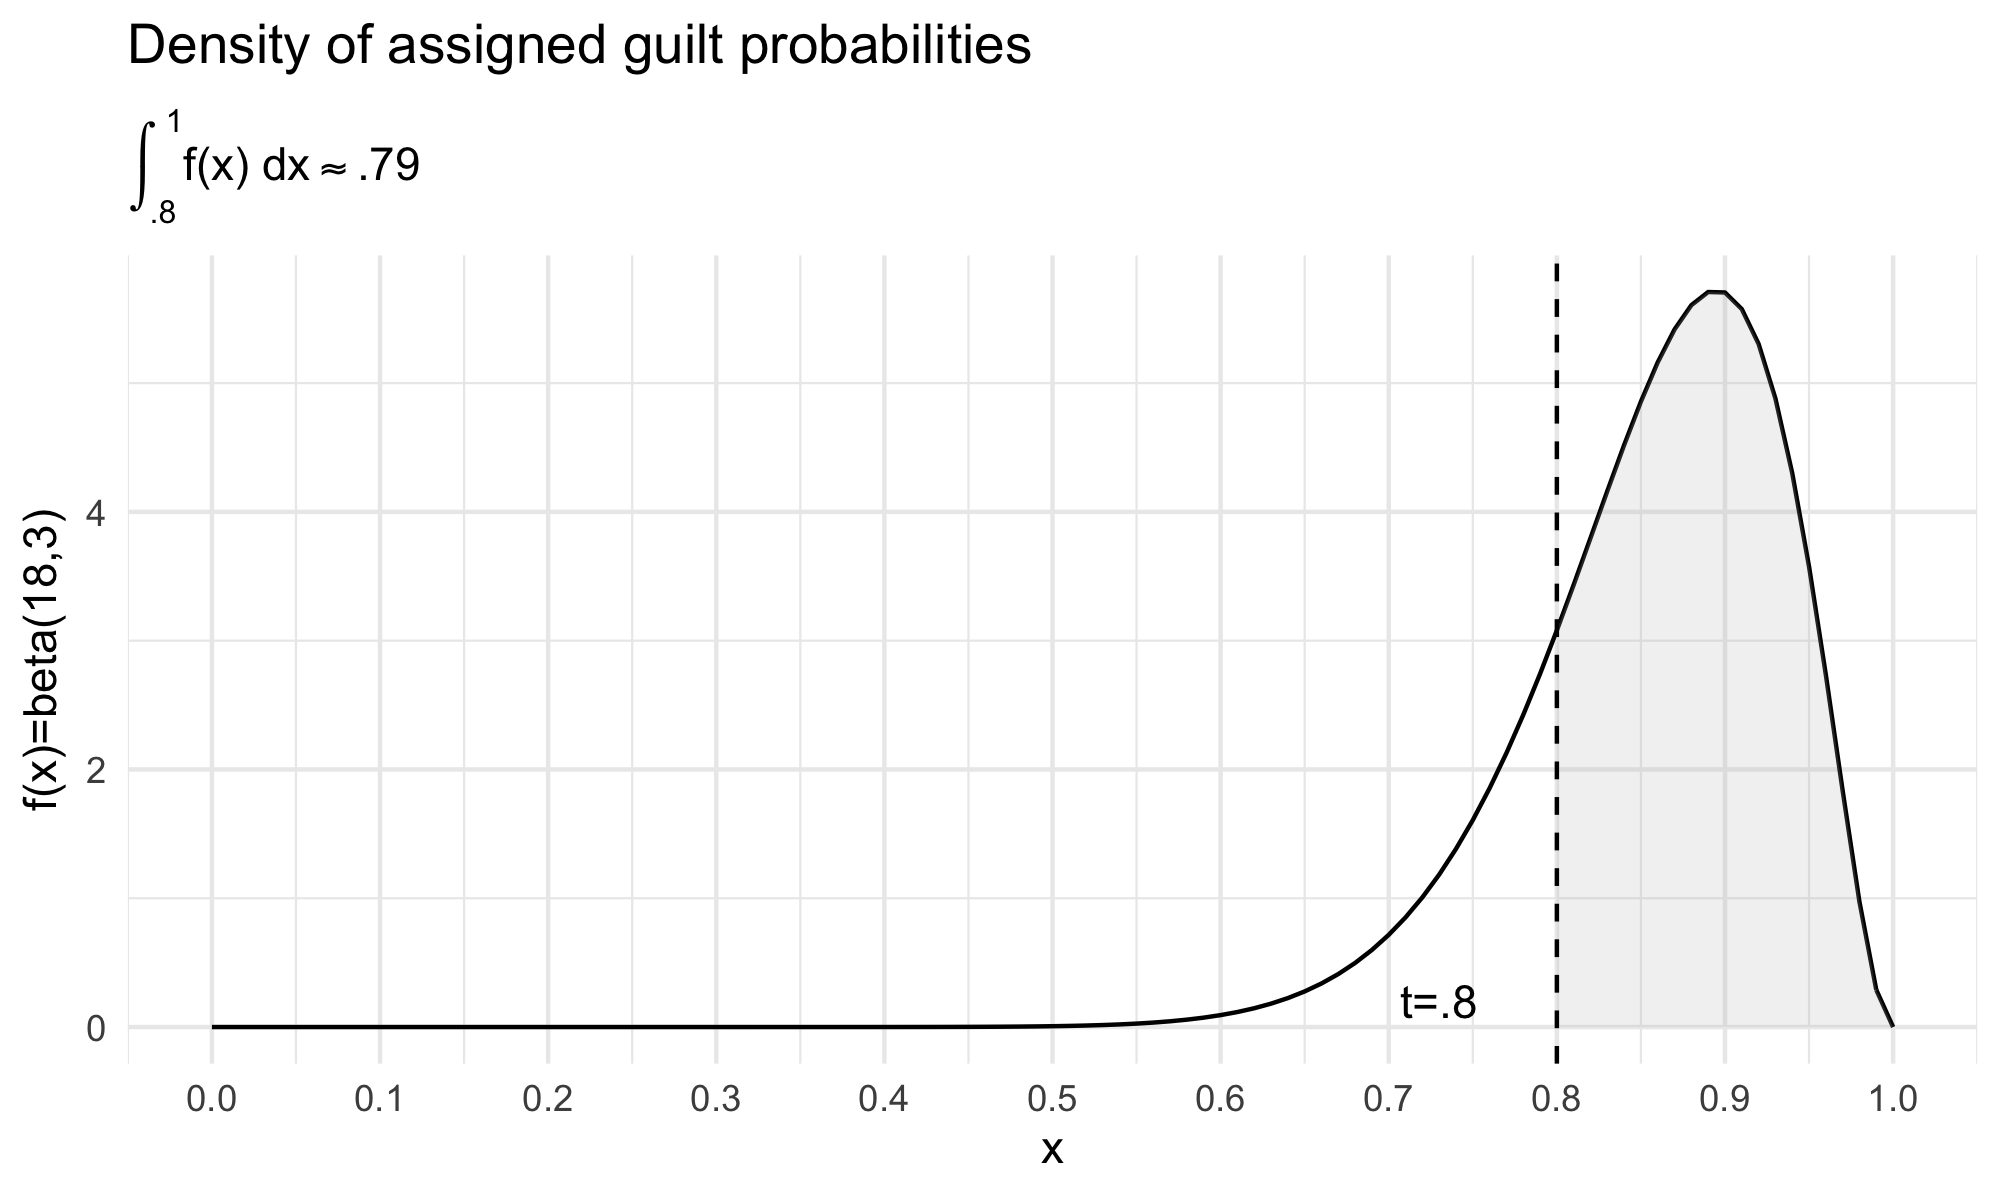
\includegraphics[width=10cm]{beta(18,3)2.png}
\end{center}

\noindent What does the distribution represent? Does it represent the
probability of guilt assigned to defendants at the beginning or the end
of the trial? There should be a difference between the
two---hopefully---or else trial proceedings would be useless. Suppose
that the distribution represents the guilt probabilities as they are
assigned to defendants at the end of the trial, once all the evidence,
counterevidence, arguments and counterarguments have been proferred and
weighed appropriately.

The choice of the distribution is for illustrative purposes only. There
are no empirical data suggesting this is the right distribution to use.
But its choice is not arbitrary either. The right skew of the
distribution reflects the assumption that defendants in criminal cases
are prosecuted only if the incriminating evidence against them is
strong. It should be no surprise that most defendants are assigned a
high probability of guilt. This is plausible in principle. For people
should not be prosecuted if the evidence against them is weak. The
distribution of the probability of liability in civil cases over a
period of time might look quite different, perhaps centered around 50\%
or 60\%.

In the figure above, the threshold for conviction is set at \(>80\%\),
and the area under the curve to the right of the threshold is about
\(.79\). According to this model, 79\% of defendants on trial are
convicted and 21\% acquitted. These figures are close to the rates of
conviction and acquittal in many countries (REFERENCES?). Since \(f(x)\)
is a probability density, the total area under the curve adds up to 1,
encompassing all defendants, both convicted and acquitted defendants.

If the threshold becomes more stringent---for example, it moves up to
85\%---the rate of conviction would decrease. This holds provided the
underlying distribution does not change. But, if the threshold is set
higher, those who are prosecuted will tend to face comparatively
stronger evidence and thus the distribution will become more skewed
toward the right---say \textsf{beta(25,3)}. As a consequence, the rate
of conviction could still be about 79\% even with a more stringent
threshold of 85\%.

\begin{center}
    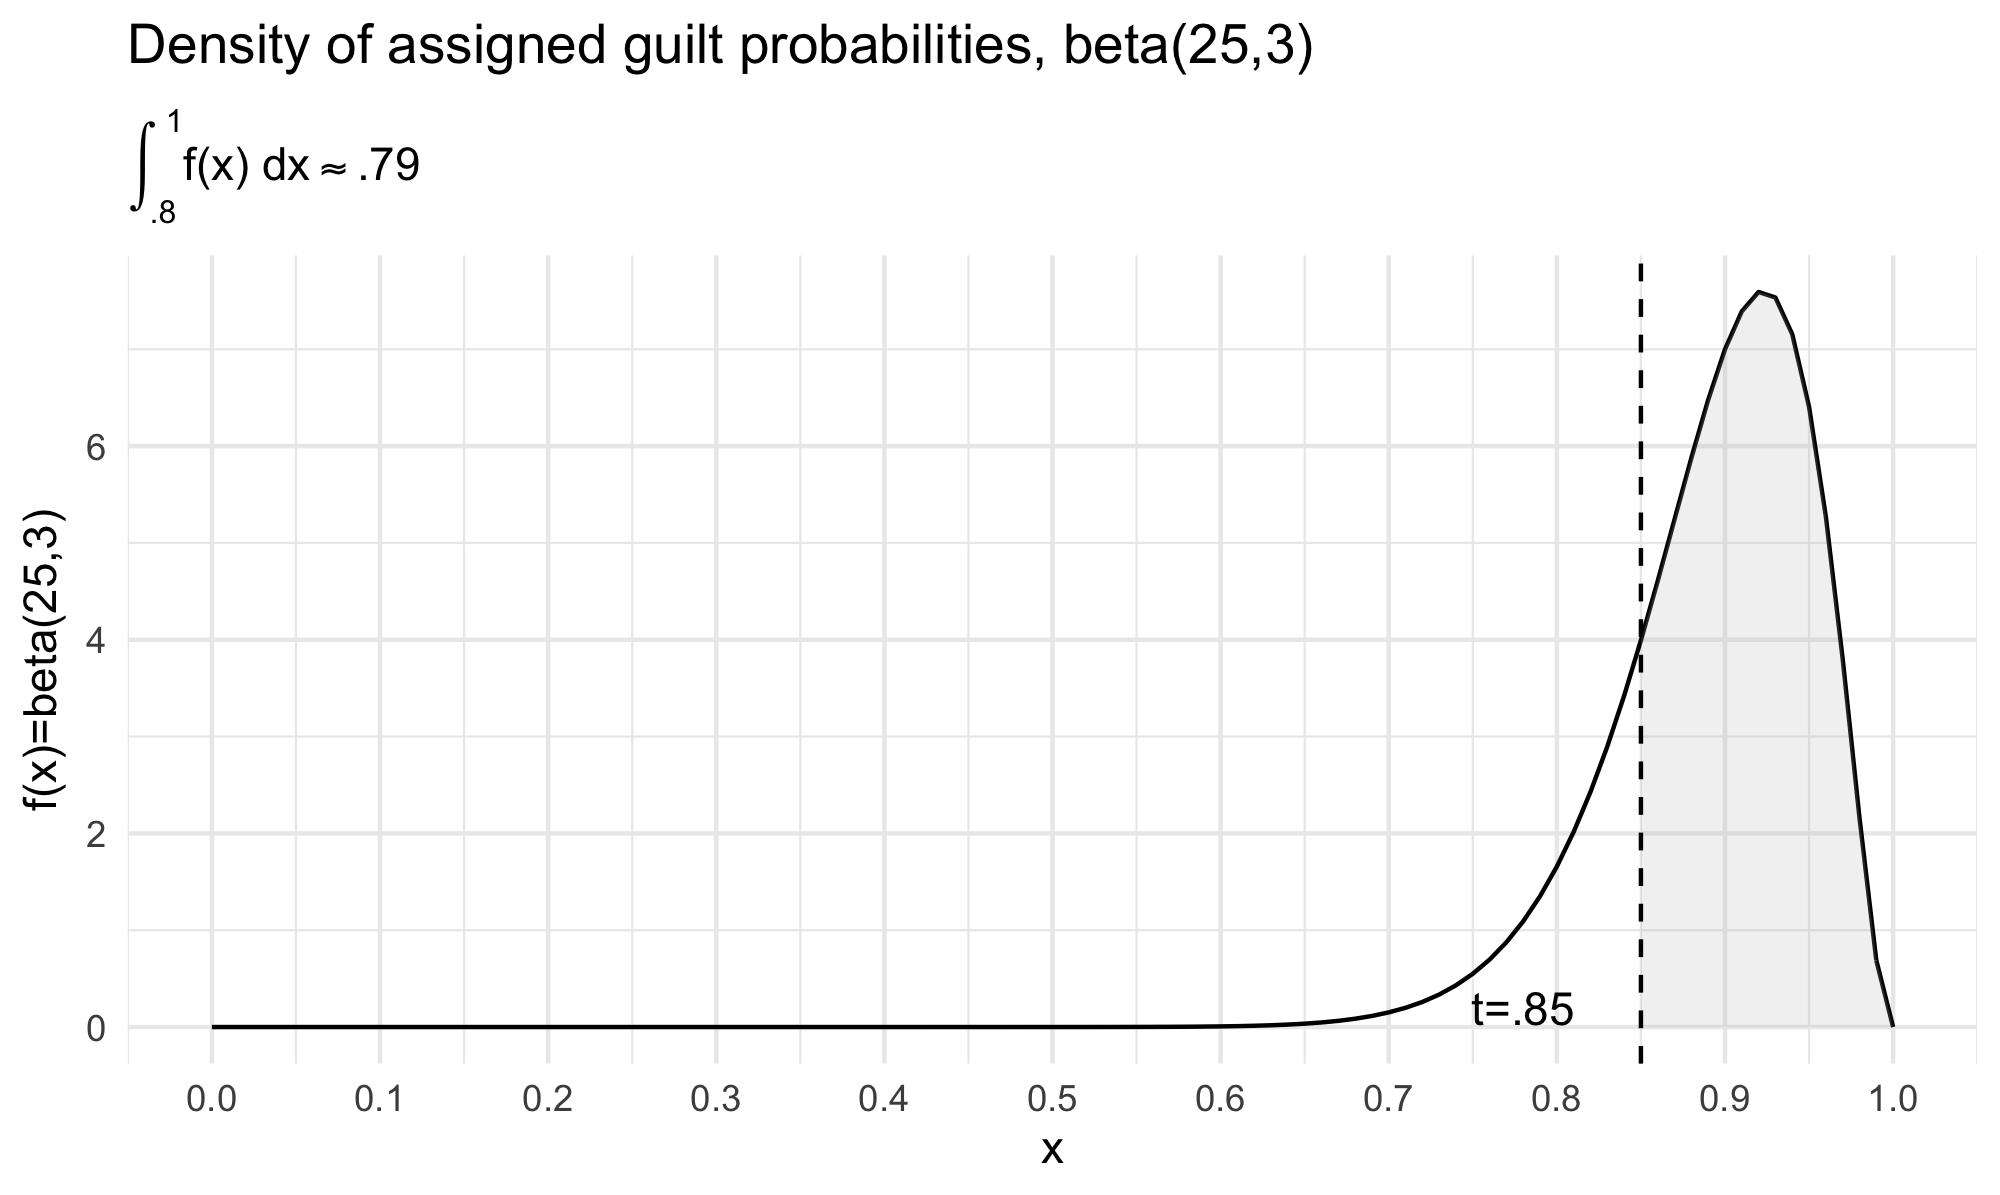
\includegraphics[width=10cm]{dbeta(25,3)2.png}
\end{center}

The two graphs above depict the rate of conviction among those who are
facing trial, not the rate of conviction in the general population
overall. As just shown, the rate of conviction could remain the same
even if the probability threhsold is made more stringent. But, the rate
of conviction in the general population is likely to diminish so long as
higher thresholds, by acting as deterrents against prosecution, make it
less likely that people would be prosecuted .

This formal model does not yet make any distinction between factually
guilt and factually innocet defendants. But, presumably, some defendants
committed the acts they are accused of and others did not. This is not a
clear-cut distinction, however. Some defendants may have committed the
acts they are accused of to some extent, but not to the full extent they
are accused of, while others may be completely innocent of any crime
whatsoever. Leaving this subtlety aside, the formal model can be refined
to distinguish between factually innocent and guilty defendants.

The simplest refinement would create two separate distributions, one
distribution for the factually innocent defendants and the other for the
factually guilty defendants. The problem with this is that we have
little idea about what these distributions should look like in the first
place. Hopefully, the innocent distribution will be more left skewed and
the guilty distribution more right skewed. Guilty defendants should be
assigned, on average, higher guilt probabilities than innocent
defendants. The two distributions could still overlap to some extent as
some guilt defendants could be assigned as low guilt probabilities as
some innocent defendants and conversely some innocent defendants could
be assigned as high guilt probabilities as some guilty defendants. This
is unfortunate, but also an inevitable consequence of the fallibility of
the trial system.

A more principled way to add two separate distributions to the model,
one for guilty and another for innocent defendants, would be to derive
them from the overall distribution of defendants. This can be done by
following the simple principle that, among those defendants who are
assigned a probability of, say, 80\%, there should be a corresponding
proportion of 80\% guilty people and 20\% innocent people. These are of
coruse expected values, not actual values. Say you are throwing a fair
six-faced die. In the long run, you would expect that in 1/6 of the
throws the die would land, say on ``4.''

The expected proportion of guilty and innocent defendants on trial, out
of all defendants, can be inferred from the density distribution
\(f(x)\) under certain assumptions. Suppose each defendant is assigned a
guilt probability based on the best and most complete evidence. From the
perspective of judges and jurors (or anyone who has access to the
evidence and evaluates it the same way), \(x\%\) of defendants who are
assigned \(x\%\) guilt probability are expected to be guilty and
\((1-x)\%\) innocent. For example, 85\% of defendants who are assigned a
85\% guilt probability are expected to be guilty and 15\% innocent; 90\%
of defendants who are assigned a 90\% guilt probability are expected to
be guilty and 10\% innocent; and so on.

So the expected guilty distribution as a function of \(x\) will be
\(x f(x)\), while the expected innocent distribution will be
\((1-x)f(x)\). In other words, the function \(xf(x)\) describes the
(expected) assignment of guilt probabilities for guilty defendants, and
similarly, \((1-x)f(x)\) the (expected) assignment of guilt
probabilities for innocent defendants. Neither of these functions is a
probability density, since \%\(\int_0^1 \! xf(x) \, \mathrm{d}x=0.86\)
and \(\int_0^1 \! (1-x)f(x) \, \mathrm{d}x=0.14\). These numbers express
the (expected) proportion of guilty and innocent defendants out of all
defendants on trial, respectively 86\% and 14\%.

The rates of incorrect decisions---false convictions and false
acquittals or more generally false positives and false negatives---can
be inferred from this model as a function of the threshold \(t\) (Hamer,
2004, 2014). The integral \(\int_0^t \! xf(x) \, \mathrm{d}x\) equals
the expected rate of false acquittals, or in other words, the expected
proportion of guilty defendants who fall below threshold \(t\) (out of
all defendants), and the integral
\(\int_t^1 \! (1-x)f(x) \, \mathrm{d}x\) equals the expected rate of
false convictions, or in other words, the expected proportion of
innocent defendants who fall above threshold \(t\) (out of all
defendants). The rates of correct decisions---true convictions and true
acquittals or more generally true positives and true negatives---can be
inferred in a similar manner. The integral
\(\int_t^1 \! xf(x) \, \mathrm{d}x\) equals the expected rate of true
convictions and \(\int_0^t \! (1-x)f(x) \, \mathrm{d}x\) the expected
rate of true acquittals. In the figure below, the regions shaded in gray
correspond to false negatives (false acquittals) and false positives
(false convictions). The remaining white regions within the solid black
curve correspond to true positives (true convictions) and true negatives
(true acquittals). Note that the dotted blue curve is the original
overall distribution for all defendants.

\begin{center}
    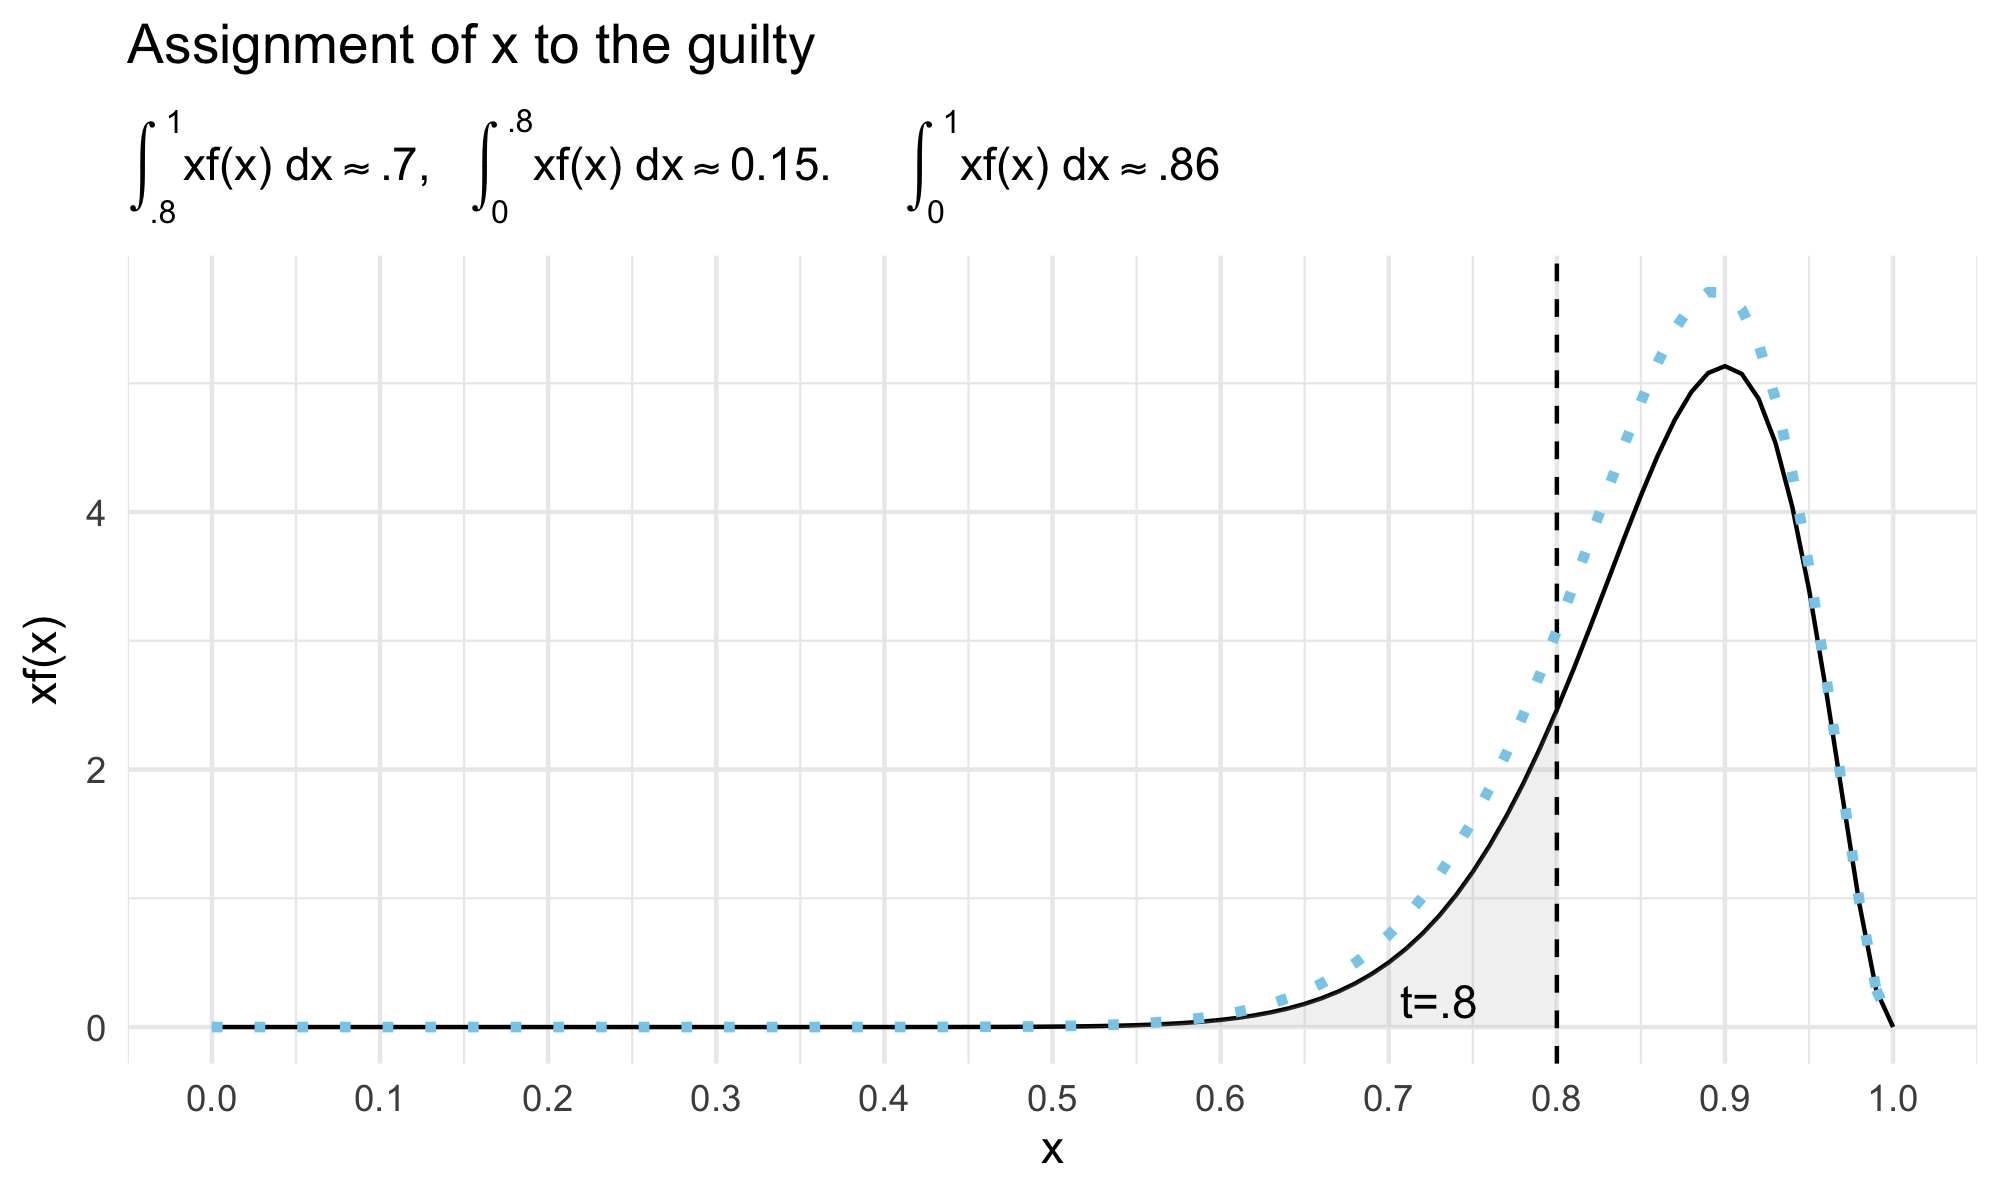
\includegraphics[width=10cm]{xfx3.png}
\end{center}

\begin{center}
    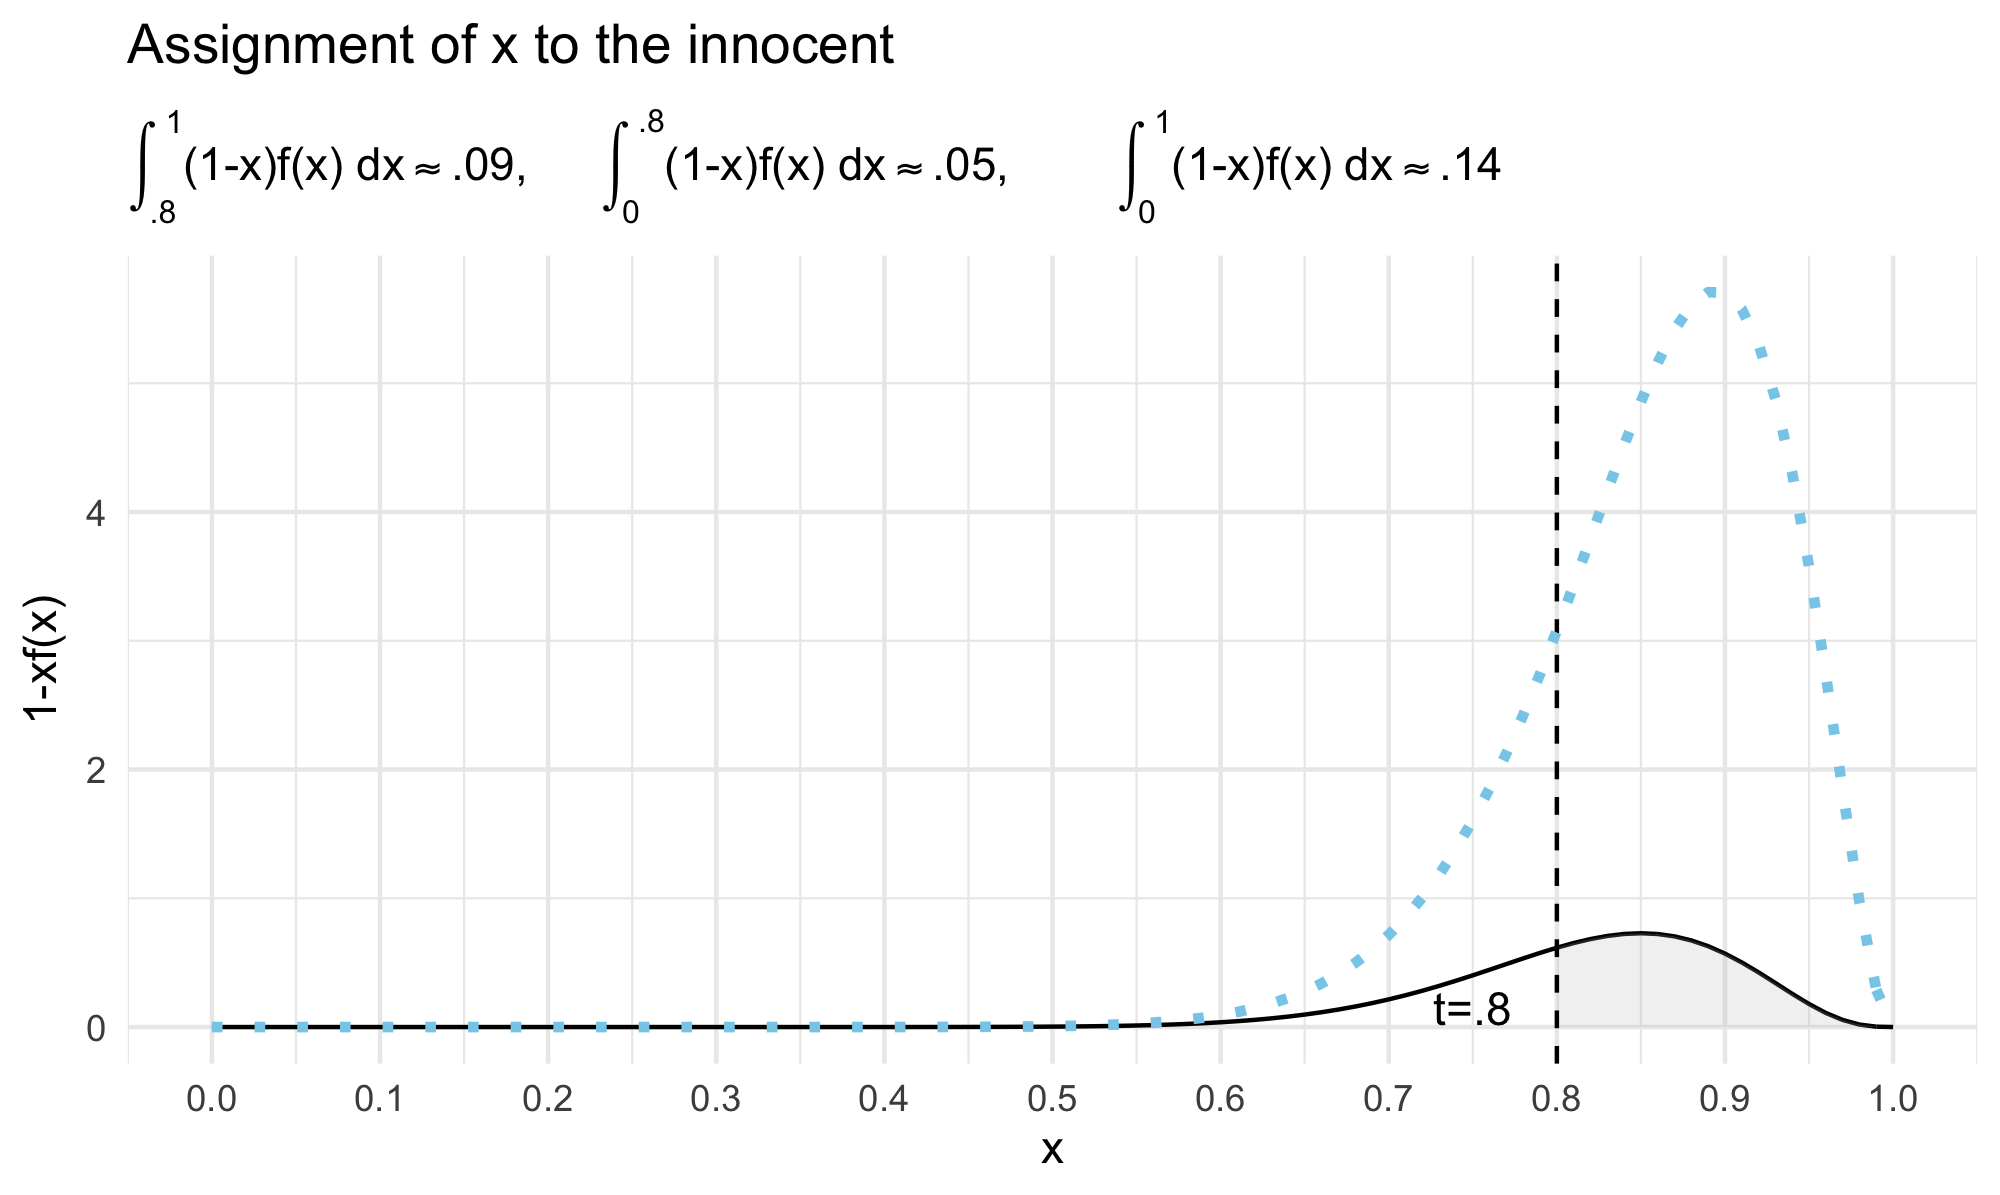
\includegraphics[width=10cm]{nxfx3.png}
\end{center}

The size of the grey regions in the figures above---which correspond to
false positives and false negatives---is affected by the location of
threshold \(t\). As \(t\) moves upwards, the rate of false positives
decreases but the rate of false negatives increases. Conversely, as
\(t\) moves downwards, the rate of false positives increases but the
rate of false negatives decreases. This trade-off is inescapable so long
as the underlying distribution is fixed. We have already remarked on the
possibility that the distribution would change in shape as a result of
changes in the probability threhsold. We will retunr to this point later
in the chapter.

Below are both error rates---false positives and false negatives---and
their sum plotted against a choice of \(t\), while holding fixed the
density function \(\textsf{binom(18,3)}\). The graph shows that any
threshold that is no greater than 50\% would minimize the total error
rate \%(comprising false positives and false negatives). A more
stringent threshold, say \(>90\%\), would instead significantly reduce
the rate of false positives but also significantly increase the rate of
false negatives, es expected.

\begin{center}
    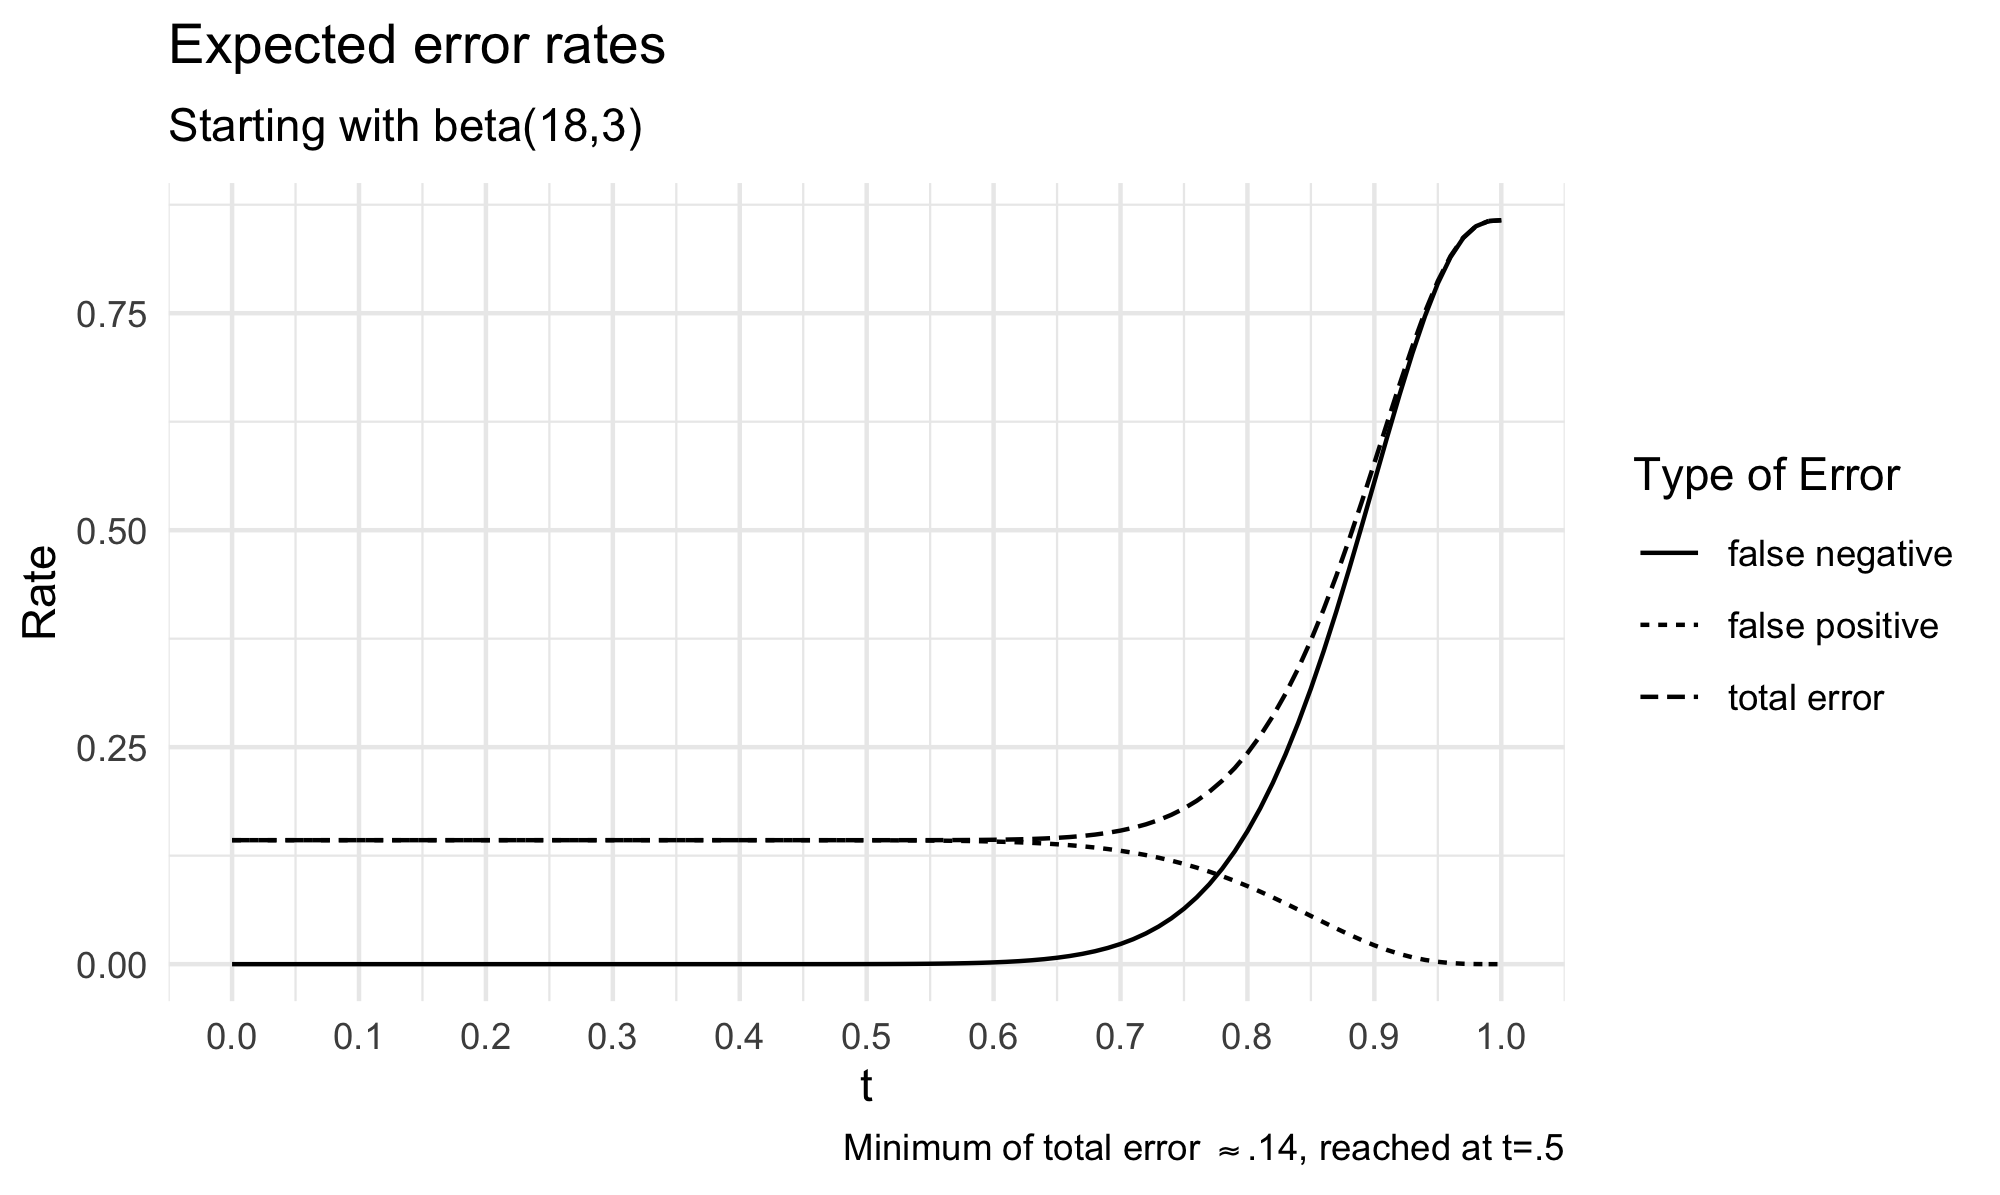
\includegraphics[width=12cm]{errors.png}
\end{center}

In general, the threshold that minimizes the expected rate of incorrect
decisions overall, no matter the underlying distribution, lies at
\(50\%\). The claim that setting threshold at \(t=.5\) minimizes the
expected error rate holds given the distribution \(f(x)=\)beta(18,3) as
well as any other distribution
\citep{kaye1982limits, Kaye1999Clarifying-the-, cheng2015}. To show
this, let \(E(t)\) \%as a function of threshold \(t\) be the sum of
rates of false positive and false negative decisions:

\[E(t) = \int_0^t \! x f(x) \, \mathrm{d}x + \int_t^1 \! (1-x) f(x) \, \mathrm{d}x.
\]

The overall rate of error is minimized when \(E(t)\) is the lowest. To
determine the value of \(t\) for which \(E(t)\) is the lowest, set the
derivative of \(E(t)\) \%and \(R(t)\) to zero, that is,
\(\frac{d}{dt} E(t)= 0\). By calculus,
\(t=1/2\).\footnote{Note that $\frac{d}{dt}  E(t)$ is the the sum of the derivatives of $\int_0^t \! x f(x) \, \mathrm{d}x$ 
and 

$\int_t^1 \!(1-x) f(x) \, \mathrm{d}x$
, that is,

\[\frac{d}{dt} E(t) = \frac{d}{dt}  \int_0^t \! x f(x) \, \mathrm{d}x + \frac{d}{dt}  \int_t^1 \! (1-x) f(x) \, \mathrm{d}x.\]

By the fundamental theorem of calculus, 

\[\frac{d}{dt}   \int_0^t \! x f(x) \, \mathrm{d}x = tf(t) \text{ and }
\frac{d}{dt}   \int_t^1 \! (1-x) f(x) \, \mathrm{d}x = -(1-t)f(t). \]

By plugging in the values, 

\[\frac{d}{dt}  E(t) = tf(t)  -(1-t)f(t). \]

Since $\frac{d}{dt}  E(t)= 0$, then $tf(t)  = (1-t)f(t)$
and thus
$t  = 1-t$, so 
$t  = 1/2$ or a $>50\%$ threshold.
} This claims holds when the two decisional errors are assigned the same
weight, or in other words, the costs of false positives and false
negatives are symmetric. The \(>50\%\) threshold therefore should be
most suitable for civil trials. In criminal trials, however, false
convictions are typically considered significantly more costly than
false acquittals, say a cost ratio of 9:1 (but see (Epps, 2015)). The
sum of the two error rates can be weighted by their respective costs:

\[E(t) = \int_0^t \! x f(x) \, \mathrm{d}x + 9\int_t^1 \! (1-x) f(x) \, \mathrm{d}x.
\]

Given a cost ratio of 9:1, the optimal threshold that minimizes the
(weighted) overall rate of error is no longer \(1/2\), but rather,
\(t=9/10=90\%\).\footnote{The proof is the same as before. Since $tf(t)  = 9(1-t)f(t)$, it follows that 
$t  = 9/10$.}

Whenever the decision threshold is more stringent than \(>50\%\), the
overall (unweighted) error minimization may be sacrificed to pursue
other goals, for example, protecting more innocents against mistaken
convictions, even at the cost of making a larger number of mistaken
trial decisions overall.

The standard `proof beyond a reasonable doubt' is often paired with the
Blackstone ratio, the principle that it is better that ten guilty
defendants go free rather than even just one innocent be convicted. The
exact ratio is a matter of controversy (Volokh, 1997). It is tempting to
think that, say, a 99\% threshold guarantees a 1:99 ratio between false
convictions and false acquittals. But this would be hasty for at least
two reasons. First, probabilistic thresholds affect the expected rate of
mistaken decisions. The actual rate may deviate from its expected value
(\textbf{Kaye1999Clarifying-the?}-). Second, if the threshold is
\(99\%\), \textit{at most} 1\% of decision against defendants are
expected to be mistaken (false convictions) and \textit{at most} 99\% of
the decisions in favor of the defendant are expected to be mistaken
(false acquittals). The exact ratio will depend on the probabilities
assigned to defendants and how they are distributed \citep{allen2014}.
The (expected) rate of false positives and false negatives---and thus
their ratio---depend on where the threshold is located but also on the
distribution of the liability probability as given by the density
function \(f(x)\).

\hypertarget{interval-thresholds-finkelstein}{%
\subsection{Interval thresholds
(Finkelstein)}\label{interval-thresholds-finkelstein}}

The prior probability cannot be easily determined (R. D. Friedman,
2000). Even if it can be determined, arriving at a posterior probability
might be impractical because of lack of adequate quantitative
information. Perhaps, decision thresholds should not rely on a unique
posterior probability but on an interval of admissible probabilities
given the evidence (Finkelstein \& Fairley, 1970). Perhaps, the
assessment of the posterior probability of guilt can be viewed as an
idealized process, a regulative ideal which can improve the precision of
legal reasoning. (CITE BIEDERMAN TARONI).

--\textgreater{}

\hypertarget{theoretical-challenges---new-chapter-would-statrt-here}{%
\section{Theoretical challenges - NEW CHAPTER WOULD STATRT
HERE}\label{theoretical-challenges---new-chapter-would-statrt-here}}

Let's take stock. We briefly examined difficulties in implementation for
probabilistic standards of proof and set those aside. We then offered a
few illustrations how probabilistic standards can be used as analytical
tools to theorize about decision-making at trial. But even if
probabilistic thresholds are used solely as analytical tools, legal
probabilists are not yet out of the woods. Even if the practical
problems can be addressed or set aside, theoretical difficulties remain.
We will focus on three in particular: the problem of priors; naked
statistical evidence; and the difficulty about conjunction, also called
the conjunction paradox. The latter two are difficulties that any theory
of the standard of proof -- not just a probabilistic theory -- should be
able to address. The first difficulty is peculiar to the probabilistic
interpretation of standards of proof. We will examine each difficulty in
turn and then examine a promising line of response within legal
probabilism based on likelihood ratios instead of posterior
probabilities.

\hypertarget{the-problem-of-priors}{%
\subsection{The problem of priors}\label{the-problem-of-priors}}

\hypertarget{naked-statistical-evidence}{%
\subsection{Naked statistical
evidence}\label{naked-statistical-evidence}}

Suppose one hundred, identically dressed prisoners are out in a yard
during recreation. Suddenly, ninety-nine of them assault and kill the
guard on duty. We know that this is what happened from a video
recording, but we do not know the identity of the ninety-nine killers.
After the fact, a prisoner is picked at random and tried. Since he is
one of the prisoners who were in the yard, the probability of his guilt
would be 99\%. But despite the high probability, many have the intuition
that this is not enough to establish guilt beyond a reasonable doubt.
Hypothetical scenarios of this sort suggest that a high probability of
guilt, while perhaps necessary, is not sufficient to establish guilt
beyond a reasonable doubt.

Perhpas, the resistance in the prisoner scenario lies in the fact that
the prisoner was picked at random, and that any prisoner would be 99\%
likely to be one of the killers. Since the statistics cannot single out
the one innocent prisoner, they are bad evidence. But consider this
case. Suppose two people enter a department store. There are no other
customers in the store. After they exit the store, a member of the staff
finds that an item of merchandise is missing. Since no staff member
could be culpable---they are strictly surveilled---the culprit must be
one of the customers. One of the customers, John, has scored high in a
compulsivity test and has been arrested for stealing in department
stores several times in the past. The other customer, Rick, has never
been arrested for stealing in a department store and shows no sign of
high compulsivity. Statistics show that people with a high degree of
compulsivity and who have stolen merchandise in department stores before
are more likely than others to steal merchandise if they are
unsupervised. So John is most likely the culprit. Suppose studies show
that people like John, when unsupervised, will steal 99 times out of 100
times. Instead, people like Rick, when unsupervised, will only steal 1
time out of 100 times. So John is 99 times more likely than Rick to have
stolen the merchandise. Can these statistics be enough to convict John?
Again, it seems not. There is no evidence against him specifically, say,
no merchandise was found on him that could link him to the crime. Many
would feel uneasy about convicting John despite the fact that, between
the two suspects, he is the one who is most likely the culprit.

A similar hypothetical can be constructed for civil cases. Suppose a bus
company, Blue-Bus, operates 90\% of the buses in town on a certain day,
while Red-Bus only 10\%. That day a bus injures a pedestrian. Although
the buses of the two companies can be easily recognized because they are
respectively painted blue and red, the pedestrian who was injured cannot
remember the color of the bus involved in the accident. No other witness
was around. Still, given the statistics about the market shares of the
two companies, it is 90\% probable that a Blue-Bus bus was involved in
the accident. This is a high probability, well above the 50\% threshold.
Yet the 90\% probability that a Blue-Bus bus was involved in the
accident would seem---at least intuitively---insufficient for a judgment
of liability against Blue-Bus. This intuition challenges the idea that
the preponderance standard in civil cases only requires that the
plaintiffi establish the facts with a probability greater than 50\%.

Confronted with these hyptheticals, legal probabilists could push back.
Hypotheticals rely on intuitive judgments, for example, that the high
probability of the prisoners's guilt in the scenario above does not
amount to proof beyond a reasonable doubt. But suppose we changed the
numbers and imagined there were one thousand prisoners of whom nine
hundred and ninety-nine killed the guard. The guilt probability of a
prisoner picked at random would be 99.9\%. Even in this situation, many
would insist that guilt has not been proven beyond a reasonable doubt
despite the extremely high probability of guilt. But others might say
that when the guilt probability reaches such extreme values, values as
high as 99.9\% or higher, people's intuitive resistance to convicting
should subside (Roth, 2010). A more general problem is that intuitions
in such hypothetical scenarios are removed from real cases and thus are
potentially unreliable as a guide to theorize about standards of proof
(Ronald J. Allen \& Leiter, 2001; Hedden \& Colyvan, 2019; Lempert,
1986).

Another reason to be suspicious of these hypotheticals is that they seem
to amplify biases in human reasoning. Say an eyewitness was present
during the accident and testified that a Blue-Bus bus was involved.
Intuitively, the testimony would be considered enough to rule against
Blue-Bus, at least provided the witness survived cross-examination. We
exhibit, in other words, an intuitive preference for judgments of
liability based on testimonial evidence compared to judgments based on
statistical evidence. This preference has been experimentally verified
(Arkes, Shoots-Reinhard, \& Mayes, 2012; Niedermeier, Kerr, \& Messeé,
1999; Wells, 1992) and exists outside the law (Ebert, Smith, \& Durbach,
2018; O. Friedman \& Turri, 2015; Sykes \& Johnson, 1999). But
testimonial evidence is no less prone to error than statistical
evidence. In fact, it may well be more prone to error. The unreliability
of eyewitness testimony is well-known, especially when the environmental
conditions are not optimal (Loftus, 1996). So are we justified in
exhibiting an intuitive preference for eyewitness testimony as opposed
to statistical evidence, or is this preference a cognitive bias to
avoid?

These reservations notwithstanding, the puzzles about naked statistical
evidence cannot be easily dismissed. Puzzles about statistical evidence
in legal proof have been around for a while (Cohen, 1977; Kaye, 1979b;
Nesson, 1979; Thomson, 1986). Philosophers and legal scholars have shown
a renewed interest in both criminal and civil cases (Blome-Tillmann,
2017; Bolinger, 2018; Cheng, 2012; Di Bello, 2019; Enoch, Spectre, \&
Fisher, 2012; Ho, 2008; Moss, 2018; Nunn, 2015; Pardo, 2018; Pritchard,
2005; Pundik, 2017; Redmayne, 2008; Roth, 2010; Smith, 2018; Stein,
2005; Wasserman, 1991). Given the growing interest in the topic, legal
probabilism cannot be a defensible theoretical position without offering
a story about naked statistical evidence.

\hypertarget{conjuction-paradox-new-chapter-here-devoted-to-probability-based-solutions}{%
\section{Conjuction paradox -- NEW CHAPTER HERE DEVOTED TO PROBABILITY
BASED
SOLUTIONS}\label{conjuction-paradox-new-chapter-here-devoted-to-probability-based-solutions}}

Another theoretical difficulty that any theory of the standard of proof
should address is the the conjunction paradox or difficulty about
conjunction. First formulated by Cohen (1977), the difficulty about
conjunction has enjoyed a great deal of scholarly attention every since
(Ronald J. Allen, 1986; Ronald J. Allen \& Stein, 2013; R. Allen \&
Pardo, 2019; Haack, 2014; Schwartz \& Sober, 2017; Stein, 2005). This
difficulty arises when an accusation of wrongdoing, in a civil or
criminal proceeding, is broken down into its constituent elements. The
basic problem is that the probability of a conjuction is often lower
than the probability of the conjuncts. Thus, even if each conjunct meets
the requisite probability threshold, the conjunction does not. This
chapter examines the difficulty about conjuction and how legal
probabilists can respond.

\hypertarget{the-problem}{%
\subsection{The problem}\label{the-problem}}

Suppose that in order to prevail in a criminal trial, the prosecution
should establish by the required standard, first, that the defendant
caused harm to the victim (call it claim \(A\)), and second, that the
defendant had premeditated the harmful act (call it claim \(B\)). Cohen
(1977) argues that common law systems subscribe to a conjunction
principle, that is, if \(A\) and \(B\) are established according to the
governing standard of proof, so is their conjunction (and vice versa).
If the conjunction principle holds, the following must be equivalent,
where \(S\) is a placeholder for the standard of proof:

\begin{center}
\begin{tabular}
{@{}ll@{}}
\toprule
\textbf{Separate} &   A is established according to S and B is established according to S\\   
\textbf{Overall}  &   The conjunction $A \et B$ is established according to S  \\ 
\bottomrule
\end{tabular}
\end{center}

\noindent Let \(S[X]\) mean that claim or hypothesis \(X\) is
established according to standard \(S\). Then, in other words, the
conjunction principles requires that:
\[S[A \wedge B] \Leftrightarrow S[A] \wedge S[B].\]

The conjunction principle is consistent with---perhaps even required
by---the case law. For example, the United States Supreme Court writes
that in criminal cases

\begin{quote}
the accused [is protected] against conviction except upon proof beyond a reasonable doubt of \textit{every fact} necessary to constitute the crime with which he is charged. In re Winship (1970), 397 U.S. 358, 364. 
\end{quote}

\noindent A plausible way to interpret this quotation is to posit this
identity: to establish someone's guilt beyond a reasonable doubt
\textit{just is} to establish each element of the crime beyond a
reasonable doubt. Thus,

\begin{align*}\mathsf{BARD}[A_1 \wedge \cdots \wedge A_n] \Leftrightarrow \mathsf{BARD}[A_1] \wedge \cdots \wedge \mathsf{BARD}[A_n],
\end{align*}

\noindent where the conjunction \(A_1 \et \cdots \et A_n\) comprises all
the material facts that, according to the applicable law, constitute the
crime with with the accused is charged.

The problem for the legal probabilist is that the conjunction principle
conflicts with a threshold-based probabilistic interpretation of the
standard of proof. For suppose the prosecution presents evidence that
establishes claims \(A\) and \(B\), separately, to the required
probability, say about 95\% each. Has the prosecution met the burden of
proof? Each claim was established to the requisite probability
threshold, and thus it was established to the requisite standard
(assuming the threshold-based interpretation of the standard of proof).
And if each claim was established to the requisite standard, then (i)
guilt as a whole was established to the requisite standard (assuming the
conjunction principle). But even though each claim was established to
the requisite probability threshold, the probability of their
conjunction---assuming the two claims are independent---is only
\(95\%\times95\%=90.25\%\), below the required 95\% threshold. So (ii)
guilt as a whole was \textit{not} established to the requisite standard
(assuming a threshold-based probabilistic interpretation of the
standard). Hence, we arrive at two contradictory conclusions: (i) that
the prosecution met its burden of proof and (ii) that it did not meet
its burden.

The difficulty about conjunction---the fact that a probabilistic
interpretation of the standard of proof conflicts with the conjunction
principle---does not subside when the number of constituent claims
increases. If anything, the difficulty becomes more apparent. Say the
prosecution has established three separate claims to 95\% probability.
Their conjunction---again if the claims are independent---would be about
85\% probable, even further below the 95\% threshold. Nor does the
difficulty about conjunction subside if the claims are no longer
regarded as independent. The probabilty of the conjunction \(A \et B\),
without the assumption of independence, equals
\(\pr{A | B} \times \pr{B}\). But if claims \(A\) and \(B\), separately,
have been established to 95\% probability, enough for each to meet the
threshold, the probability of \(A \et B\) could still be below the 95\%
threshold unless \(\pr{A | B}=100\%\). For example, that someone
premediated a harmful act against another (claim \(B\)) makes it more
likely that they did cause harm in the end (claim \(A\)). Since
\(\pr{A | B} > \pr{A}\), the two claims are not independent. Still,
premeditation does not always lead to harm, so \(\pr{A | B}\) should be
below 100\%. Consequently, in this case, the probability of the
conjunction \(A \et B\) would be below the 95\%
threhsold.\todo{False in whole generality, give a counterexample with more specific numbers. M: I changed things a bit. Maybe not it's clear now. The counterexample is basically P(A)=P(B)=0.95, but P(AB)=Pr(A)*P(A|B) and since P(A|B) is below 1, then P(AB) is below 0.95.}

\hypertarget{references}{%
\section*{References}\label{references}}
\addcontentsline{toc}{section}{References}

\hypertarget{refs}{}
\begin{CSLReferences}{1}{0}
\leavevmode\hypertarget{ref-Allen1986A-Reconceptuali}{}%
Allen, Ronald J. (1986). A reconceptualization of civil trials.
\emph{Boston University Law Review}, \emph{66}, 401--437.

\leavevmode\hypertarget{ref-allen2001naturalized}{}%
Allen, Ronald J., \& Leiter, B. (2001). Naturalized epistemology and the
law of evidence. \emph{Virginia Law Review}, \emph{87}(8), 1491--1550.

\leavevmode\hypertarget{ref-allen2013}{}%
Allen, Ronald J., \& Stein, A. (2013). Evidence, probability and the
burden of proof. \emph{Arizona Law Journal}, \emph{55}, 557--602.

\leavevmode\hypertarget{ref-AllenPardo2019relative}{}%
Allen, R., \& Pardo, M. (2019). Relative plausibility and its critics.
\emph{The International Journal of Evidence {\&} Proof}, \emph{23}(1-2),
5--59. \url{https://doi.org/10.1177/1365712718813781}

\leavevmode\hypertarget{ref-arkesEtAl2012}{}%
Arkes, H. R., Shoots-Reinhard, B. L., \& Mayes, R. S. (2012).
Disjunction between probability and verdict in juror decision making.
\emph{Journal of Behavioral Decision Making}, \emph{25}(3), 276--294.

\leavevmode\hypertarget{ref-Bernoulli1713Ars-conjectandi}{}%
Bernoulli, J. (1713). \emph{Ars conjectandi}.

\leavevmode\hypertarget{ref-BlomeTillmann2017}{}%
Blome-Tillmann, M. (2017). {`{M}ore likely than not'} --- {K}nowledge
first and the role of bare statistical evidence in courts of law. In A.
Carter, E. Gordon, \& B. Jarvi (Eds.), \emph{Knowledge
first---approaches in epistemology and mind} (pp. 278--292). Oxford
University Press.
\url{https://doi.org/10.1093/oso/9780198716310.003.0014}

\leavevmode\hypertarget{ref-bolinger2018rational}{}%
Bolinger, R. J. (2018). The rational impermissibility of accepting
(some) racial generalizations. \emph{Synthese}, 1--17.

\leavevmode\hypertarget{ref-buchak2014belief}{}%
Buchak, L. (2014). Belief, credence, and norms. \emph{Philosophical
Studies}, \emph{169}(2), 285--311.

\leavevmode\hypertarget{ref-cheng2012reconceptualizing}{}%
Cheng, E. (2012). Reconceptualizing the burden of proof. \emph{Yale LJ},
\emph{122}, 1254.

\leavevmode\hypertarget{ref-Cohen1977The-probable-an}{}%
Cohen, J. L. (1977). \emph{The probable and the provable}. Oxford
University Press. \url{https://doi.org/10.2307/2219193}

\leavevmode\hypertarget{ref-Dekay1996}{}%
Dekay, M. L. (1996). The difference between {B}lackstone-like error
ratios and probabilistic standards of proof. \emph{Law and Social
Inquiry}, \emph{21}, 95--132.

\leavevmode\hypertarget{ref-dhamiEtAl2015}{}%
Dhami, M. K., Lundrigan, S., \& Mueller-Johnson, K. (2015). Instructions
on reasonable doubt: Defining the standard of proof and the jurors task.
\emph{Psychology, Public Policy, and Law, 21(2), 169178}, \emph{21}(2),
169--178.

\leavevmode\hypertarget{ref-diBello2019}{}%
Di Bello, M. (2019). Trial by statistics: Is a high probability of guilt
enough to convict? \emph{Mind}.

\leavevmode\hypertarget{ref-diamond90}{}%
Diamond, H. A. (1990). Reasonable doubt: To define, or not to define.
\emph{Columbia Law Review}, \emph{90}(6), 1716--1736.

\leavevmode\hypertarget{ref-ebert2018}{}%
Ebert, P. A., Smith, M., \& Durbach, I. (2018). Lottery judgments: A
philosophical and experimental study. \emph{Philosophical Psychology},
\emph{31}(1), 110--138.

\leavevmode\hypertarget{ref-Enoch2012Statistical}{}%
Enoch, D., Spectre, L., \& Fisher, T. (2012). Statistical evidence,
sensitivity, and the legal value of knowledge. \emph{Philosophy and
Public Affairs}, \emph{40}(3), 197--224.

\leavevmode\hypertarget{ref-epps2015}{}%
Epps, D. (2015). The consequences of error in criminal justice.
\emph{Harvard Law Review}, \emph{128}(4), 1065--1151.

\leavevmode\hypertarget{ref-finkelstein1970bayesian}{}%
Finkelstein, M. O., \& Fairley, W. B. (1970). A bayesian approach to
identification evidence. \emph{Harvard Law Review}, 489--517.

\leavevmode\hypertarget{ref-friedman2015}{}%
Friedman, O., \& Turri, J. (2015). Is probabilistic evidence a source of
knowledge? \emph{Cognitive Science}, \emph{39}(5), 1062--1080.

\leavevmode\hypertarget{ref-Friedman2000presumption}{}%
Friedman, R. D. (2000). A presumption of innocence, not of even odds.
\emph{Stanford Law Review}, \emph{52}(4), 873--887.

\leavevmode\hypertarget{ref-haack2011legal}{}%
Haack, S. (2014). Legal probabilism: An epistemological dissent. In
\emph{{Haack2014-HAAEMS}} (pp. 47--77).

\leavevmode\hypertarget{ref-hamer2004}{}%
Hamer, D. (2004). Probabilistic standards of proof, their complements
and the errors that are expected to flow from them. \emph{University of
New England Law Journal}, \emph{1}(1), 71--107.

\leavevmode\hypertarget{ref-hamer2014}{}%
Hamer, D. (2014). Presumptions, standards and burdens: Managing the cost
of error. \emph{Law, Probability and Risk}, \emph{13}, 221--242.

\leavevmode\hypertarget{ref-HeddenColyvan2019legal}{}%
Hedden, B., \& Colyvan, M. (2019). Legal probabilism: A qualified
defence. \emph{Journal of Political Philosophy}, \emph{27}(4), 448--468.
\url{https://doi.org/10.1111/jopp.12180}

\leavevmode\hypertarget{ref-ho2008philosophy}{}%
Ho, H. L. (2008). \emph{A philosophy of evidence law: Justice in the
search for truth}. Oxford University Press.

\leavevmode\hypertarget{ref-Horowitz1996}{}%
Horowitz, I. A., \& Kirkpatrick, L. C. (1996). A concept in search of a
definition: The effect of reasonable doubt instrcutions on certainty of
guilt standards and jury verdicts. \emph{Law and Human Behaviour},
\emph{20}(6), 655--670.

\leavevmode\hypertarget{ref-Kaplan1968decision}{}%
Kaplan, J. (1968). Decision theory and the fact-finding process.
\emph{Stanford Law Review}, \emph{20}(6), 1065--1092.

\leavevmode\hypertarget{ref-kaplow2012}{}%
Kaplow, L. (2012). Burden of proof. \emph{Yale Law Journal},
\emph{121}(4), 738--1013.

\leavevmode\hypertarget{ref-kaye79}{}%
Kaye, D. H. (1979a). The laws of probability and the law of the land.
\emph{The University of Chicago Law Review}, \emph{47}(1), 34--56.

\leavevmode\hypertarget{ref-Kaye79gate}{}%
Kaye, D. H. (1979b). The paradox of the {G}atecrasher and other stories.
\emph{The Arizona State Law Journal}, 101--110.

\leavevmode\hypertarget{ref-Laplace1814}{}%
Laplace, P.-S. (1814). \emph{Essai philosophique sur les probabilités}.

\leavevmode\hypertarget{ref-laudan2006truth}{}%
Laudan, Larry. (2006). \emph{Truth, error, and criminal law: An essay in
legal epistemology}. Cambridge University Press.

\leavevmode\hypertarget{ref-laudan2016law}{}%
Laudan, L. (2016). \emph{The law's flaws: Rethinking trials and errors?}
College Publications. Retrieved from
\url{https://books.google.pl/books?id=MvkWvgAACAAJ}

\leavevmode\hypertarget{ref-Lempert1986}{}%
Lempert, R. O. (1986). The new evidence scholarship: Analysing the
process of proof. \emph{Boston University Law Review}, \emph{66},
439--477.

\leavevmode\hypertarget{ref-Loftus1996}{}%
Loftus, E. F. (1996). \emph{Eyewitness testimony (revised edition)}.
Harvard University Press.

\leavevmode\hypertarget{ref-moss2018}{}%
Moss, S. (2018). \emph{Probabilistic knowledge}. Oxford University
Press.

\leavevmode\hypertarget{ref-Nesson1979Reasonable-doub}{}%
Nesson, C. R. (1979). Reasonable doubt and permissive inferences: The
value of complexity. \emph{Harvard Law Review}, \emph{92}(6),
1187--1225. \url{https://doi.org/10.2307/1340444}

\leavevmode\hypertarget{ref-newman1993}{}%
Newman, J. O. (1993). Beyon {``reasonable doub.''} \emph{New York
University Law Review}, \emph{68}(5), 979--1002.

\leavevmode\hypertarget{ref-niedermeierEtAl1999}{}%
Niedermeier, K. E., Kerr, N. L., \& Messeé, L. A. (1999). Jurors' use of
naked statistical evidence: Exploring bases and implications of the
{Wells} effect. \emph{Journal of Personality and Social Psychology},
\emph{76}(4), 533--542.

\leavevmode\hypertarget{ref-nunn2015}{}%
Nunn, A. G. (2015). The incompatibility of due process and naked
statistical evidence. \emph{Vanderbilt Law Review}, \emph{68}(5),
1407--1433.

\leavevmode\hypertarget{ref-pardo2018}{}%
Pardo, M. S. (2018). Safety vs.~Sensitivity: Possible worlds and the law
of evidence. \emph{Legal Theory}, \emph{24}(1), 50--75.

\leavevmode\hypertarget{ref-picinali2013}{}%
Picinali, F. (2013). Two meanings of ``reasonableness": Dispelling the
``floating" reasonable doubt. \emph{Modern Law Review}, \emph{76}(5),
845--875.

\leavevmode\hypertarget{ref-Posner1973}{}%
Posner, R. (1973). \emph{The economic analysis of law}. Brown \&
Company.

\leavevmode\hypertarget{ref-pritchard2005epistemic}{}%
Pritchard, D. (2005). \emph{Epistemic luck}. Clarendon Press.

\leavevmode\hypertarget{ref-pundik2017}{}%
Pundik, A. (2017). Freedom and generalisation. \emph{Oxford Journal of
Legal Studies}, \emph{37}(1), 189--216.

\leavevmode\hypertarget{ref-redmayne2008exploring}{}%
Redmayne, M. (2008). Exploring the proof paradoxes. \emph{Legal Theory},
\emph{14}(4), 281--309.

\leavevmode\hypertarget{ref-Roth2010}{}%
Roth, A. (2010). Safety in numbers? {D}eciding when {DNA} alone is
enough to convict. \emph{New York University Law Review}, \emph{85}(4),
1130--1185.

\leavevmode\hypertarget{ref-schwartz2017ConjunctionProblemLogic}{}%
Schwartz, D. S., \& Sober, E. R. (2017). The {Conjunction Problem} and
the {Logic} of {Jury Findings}. \emph{William \& Mary Law Review},
\emph{59}(2), 619--692.

\leavevmode\hypertarget{ref-smith2017}{}%
Smith, M. (2018). When does evidence suffice for conviction?
\emph{Mind}, \emph{127}(508), 1193--1218.

\leavevmode\hypertarget{ref-Stein05}{}%
Stein, A. (2005). \emph{Foundations of evidence law}. Oxford University
Press.

\leavevmode\hypertarget{ref-sykes1999}{}%
Sykes, D. L., \& Johnson, J. T. (1999). Probabilistic evidence versus
the representation of an event: The curious case of {Mrs.} {Prob}'s dog.
\emph{Basic and Applied Social Psychology}, \emph{21}(3), 199--212.

\leavevmode\hypertarget{ref-taroni2006bayesian}{}%
Taroni, F., Biedermann, A., Bozza, S., Garbolino, P., \& Aitken, C.
(2014). \emph{Bayesian networks for probabilistic inference and decision
analysis in forensic science} (2nd ed.). John Wiley \& Sons.

\leavevmode\hypertarget{ref-thomson1986liability}{}%
Thomson, J. J. (1986). Liability and individualized evidence. \emph{Law
and Contemporary Problems}, \emph{49}(3), 199--219.

\leavevmode\hypertarget{ref-tribe1971trial}{}%
Tribe, L. H. (1971). Trial by mathematics: Precision and ritual in the
legal process. \emph{Harvard Law Review}, \emph{84}(6), 1329--1393.

\leavevmode\hypertarget{ref-voloch1997}{}%
Volokh, A. (1997). {N} guilty men. \emph{University of Pennsylvania Law
Review}, \emph{146}(2), 173--216.

\leavevmode\hypertarget{ref-walen2015}{}%
Walen, A. (2015). Proof beyond a reasonable doubt: A balanced
retributive account. \emph{Louisiana Law Review}, \emph{76}(2),
355--446.

\leavevmode\hypertarget{ref-wasserman1991morality}{}%
Wasserman, D. T. (1991). The morality of statistical proof and the risk
of mistaken liability. \emph{Cardozo L. Rev.}, \emph{13}, 935.

\leavevmode\hypertarget{ref-wells1992naked}{}%
Wells, G. L. (1992). Naked statistical evidence of liability: Is
subjective probability enough? \emph{Journal of Personality and Social
Psychology}, \emph{62}(5), 739--752.
\url{https://doi.org/10.1037/0022-3514.62.5.739}

\end{CSLReferences}

\end{document}
